
\chapter{Runtime Enforcement Framework}
\graphicspath{{Chapter_2/Vector/}{Chapter_2/}}

Before delving into the specific details of the runtime enforcement framework, it is important to first establish some foundational concepts and the necessary notation. This section introduces key elements such as edit functions, runtime enforcement for synchronous programs, and the framework for policies defined as safety automata. Understanding these preliminaries will provide the necessary context for the subsequent discussions on the design and application of runtime enforcement mechanisms in various program types.


\section{Preliminaries and Notation}
\rhead{Preliminaries and Notation}
\label{prelim}

In this section, we introduce the notations and the safety automaton formalism used to define policies to be monitored and enforced. We also briefly recall the RE problem for synchronous programs (all the constraints that an enforcer should fulfill). 

A finite word over a finite alphabet $\Sigma$ is a finite sequence $\sigma = a_1\cdot a_2\cdots a_n$ of members of $\Sigma$, and $\Sigma^*$ denotes the set of finite words over $\Sigma$.
Considering a finite word $\sigma$, its length is denoted as  $|\sigma|$.
$\epsilon_\Sigma$ is used to denote the empty word over $\Sigma$ is denoted by $\epsilon_\Sigma$, or $\epsilon$ (when the context makes it evident).
Given two words $\sigma$ and $\sigma'$, their {\em concatenation} is indicated as $\sigma\cdot \sigma'$. 
A word $\sigma'$ is a {\em prefix} of a word $\sigma$, represented as $\sigma' \pref \sigma$, whenever a word $\sigma''$ is present such that $\sigma = \sigma'\cdot \sigma''$; $\sigma$ is called an \emph{extension} of $\sigma'$.

A reactive system with a finite {ordered} sets of Boolean inputs $I= \{i_1, i_2,\cdots,i_n\}$ and Boolean outputs $O= \{o_1, o_2,\cdots,o_m\}$ is considered.
$\Sigma_I=2^I$ denotes the input alphabet, $\Sigma_O=2^O$ denotes the output alphabet, and the input-output alphabet is $\Sigma= \Sigma_I \times \Sigma_O$.
A bit-vector/complete monomial will be used to represent each input (resp. output) event.
For example, let us consider $I=\{P, Q\}$.
Then, the input $\{P\} \in \Sigma_I$ is denoted as  $10$, while $\{Q\} \in \Sigma_I$ is denoted as $01$ and  $\{P, Q\} \in \Sigma_I$ is denoted as $11$.
A reaction (or input-output event) has the following structure: $(x_i, y_i)$, where $x_i \in \Sigma_I$ and $y_i \in \Sigma_O$.

Given  $\sigma= (x_1,y_1)\cdot(x_2,y_2)\cdots(x_n,y_n) \in \Sigma^*$ which is an input-output word, the input word acquired from $\sigma$ is $\sigma_I = x_1 \cdot x_2 \cdots x_n \in \Sigma_I$, which is a projection that ignores outputs and is based on inputs.
Similarly, the output word obtained from $\sigma$ is $\sigma_O = y_1 \cdot y_2 \cdots y_n \in \Sigma_O$ is the projection on outputs ignoring inputs.

\ignore{
	An execution $\sigma$ of a synchronous program $\calP$ is an infinite sequence of input-output events $\sigma\in\Sigma^{\omega}$, and the \emph{behavior} of a synchronous program $\calP$ is denoted as $\exec(\calP)\subseteq \Sigma^{\omega}$.
	The \emph{language} of $\calP$ is denoted by $\cal{L}(\cal{P})$ = $\{\sigma \in \Sigma^* | \exists \sigma' \in \exec(\calP) \wedge \sigma \pref \sigma'\}$ i.e. $\cal{L}(\cal{P})$ is the set of all finite prefixes of the sequences in $\exec(\calP)$.
}

A policy denoted as $\varphi$ (over $\Sigma$) represents a set $\calL(\varphi)\subseteq \Sigma^{*}$.
%A program $\calP \models \varphi$ iff $\calL(\calP) \subseteq  \calL(\varphi)$.
Given a word $\sigma \in \Sigma^*$, $\sigma \models \varphi$ iff $\sigma\in\calL(\varphi)$.
A {policy} $\varphi$ is {\em prefix-closed} if all prefixes of all words from
$\calL(\varphi)$ are also in $\calL(\varphi)$: $\calL(\varphi) = \{w\;|\;\exists w'\in\calL(\varphi): w\pref w'\}$.
Prefix-closed policies are the focus of this study.
Policies are formalized as safety automata, which we define next in
this section.



Synchronous programming languages~\cite{BenvenisteCEHLd03} are ideal for developing synchronous reactive systems.
They express safety properties via observers ~\cite{HalbwachsLR94}, which are statically verified (using model checking). Safety automata are analogous to observers but are enforced at runtime.

\begin{definition}[Safety Automaton]
	\label{def:SA}
	A \emph{safety automaton} (SA) $\calA =(Q, q_0, q_v, \Sigma, \xrightarrow{})$ is a tuple, where $Q$ denotes the set of states, known as \emph{locations}, $q_0 \in Q$ is a distinct starting location, $q_v \in Q$ is a distinct non-accepting (violating) location, the alphabet is $\Sigma=\Sigma_I\times\Sigma_O$, and the transition relation is $\xrightarrow{} \subseteq Q \times \Sigma \times Q$.
	Except for  $q_v$, all the other locations are accepting  (i.e., all the locations in $Q \setminus \{q_v\}$).
	Location $q_v$ is a distinct violating (trap) location, thus no transitions in $\xrightarrow{}$ from $q_v$ to a location in $Q \setminus \{q_v\}$.
	%
	Whenever there exists $(q, a, q') \in \xrightarrow{}$, we denote it as $q \xrightarrow{a} q'$.
	%
	Relation $\xrightarrow{}$ is extended to words $\sigma \in \Sigma^*$ by noting
	$q \xrightarrow{\sigma . a} q'$ whenever there exists $q''$ such that $q
	\xrightarrow{\sigma} q''$ and $q'' \xrightarrow{a} q'$.
	A location $q\in Q$ is reachable from $q_0$ if there exists a word $\sigma \in \Sigma^*$ such that $q_0
	\xrightarrow{\sigma} q$.
\end{definition}

An SA $\calA = (Q, q_0, q_v, \Sigma, \xrightarrow{})$ is \textit{deterministic} if $\forall
q \in Q, \forall a \in \Sigma, (q \xrightarrow{a} q' \land q \xrightarrow{a}
q'') \implies (q' = q'')$.
$\mathcal{A}$ is \textit{complete} if $\forall q \in Q, \forall a \in \Sigma, \exists q' \in Q, q \xrightarrow{a} q'$.
A word $\sigma$ is \textit{accepted} by $\mathcal{A}$ if there exists $q \in Q \setminus \{q_v\}$ such that $q_0
\xrightarrow{\sigma} q$.
The set of all words accepted by $\mathcal{A}$ is denoted as $\mathcal{L}(\mathcal{A})$.

\begin{remark}
	We can first determinize and complete a non-deterministic or incomplete automaton provided by the user.
	We further assume that $Q$ has no (redundant) locations that are
	unreachable from $q_0$. Hence, in the rest of this work, $\varphi$ is a safety policy specified as deterministic and complete SA $\calA_\varphi = (Q, q_0, q_v, \Sigma, \xrightarrow{})$. 
\end{remark}

The enforcer must first alter inputs from the environment in each step according to policy $\varphi$ specified as SA $\calA_\varphi$ according to the causality requirement.
As a result, we must examine the input policy obtained by projecting
on inputs from $\calA_\varphi$. 

\begin{definition}[Input SA $\calA_{\varphi_I}$]
	\label{def:inp:prop:proj:def}
	Given $\varphi\subseteq\Sigma^*$, specified as SA $\calA_{\varphi}=(Q, q_0, q_v, \Sigma, \rightarrow)$,  by discarding outputs on the transitions, input SA $\calA_{\varphi_I}=(Q, q_0, q_v, \Sigma_I, \rightarrow_I)$ is derived from $\calA_{\varphi}$.That is, for every transition  $q \xrightarrow{(x,y)} q' \in \rightarrow$ where $(x,y) \in \Sigma$, there is a transition  $q \xrightarrow{x} q' \in \rightarrow_I$, where $x \in \Sigma_I$.
	$\calL(\calA_{\varphi_I})$ is represented as $\varphi_I \subseteq \Sigma_I^*$.
\end{definition}

\begin{figure}[htb]
	%
	\centering
	\hspace{-4.0em}
	\subfloat[SA $\calA_{P}$. \label{fig:prop1}]{
		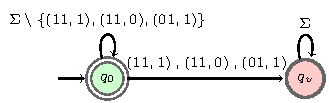
\includegraphics[scale=1]{fig/propAutomaton2-crop2.pdf}
	}
	%\hspace{1.0em}
	\subfloat[Input SA from $\calA_{P}$. \label{fig:prop1Inp}]{
		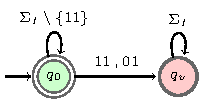
\includegraphics[scale=1]{fig/propAutomatonprojI2-crop2.pdf}
	}
	\caption[]{SA (left), and its input SA (right). \footnotemark}
	\label{fig:prop:inpProj}
\end{figure}

\footnotetext{Here, $\Sigma = \{(00,0), (00,1), (01,0), (01,1), (10,0), (10,1), (11,0), \\ (11,1)\}$. So $\Sigma \setminus \{(11,1), (11,0), (01,1)\}$ = $\{(00,0), (00,1), (01,0), (10,0), (10,1)\}$.}
%%%%%%%%%%%%%%%%%%%%%%%%%%%%%
%
%%%%%%%%%%%%%%%%%%%%%%%%%%%%%
\begin{example}[Example policy defined as SA and its input SA]
	\label{eg:prop}
	%%%%%%%%%%%%%%%%%%%%%%%%%%%%%
	Consider $I= \{B,Q\}$ and $O = \{ X \}$.
	Let us consider the policy: \textit{$P$: ``B and Q can't happen at the same time, and Q and X can't happen at the same time''}.
	Policy $P$ is defined by the safety automaton in Figure~\ref{fig:prop1}.
	The input SA for the SA in Figure~\ref{fig:prop1} defining policy $P$ is shown in Figure~\ref{fig:prop1Inp}.
	Though the SA $\calA_\varphi$ is deterministic, the input SA $\calA_{\varphi_I}$ may be non-deterministic. This is the case with the considered example as shown in Figure~\ref{fig:prop1Inp}.
\end{example} 

\begin{lemma}
	\label{lem:inputProp}
	%%%%%%%%%%%%%%%%%%%%%%%%%%%%%
	Consider $\calA_{\varphi_I}=(Q, q_0, q_v, \Sigma_I, \rightarrow_I)$ be the input automaton derived from $\calA_{\varphi}=(Q, q_0, q_v, \Sigma, \rightarrow)$. The policies we have are as follows:
	\squishlist
	\item[1] $\forall (x,y) \in \Sigma, \forall q, q'\in Q: q\xrightarrow{(x,y)}q' \implies q \xrightarrow{x}_I q'$.
	\item[2] $\forall x \in \Sigma_I, \forall q, q'\in Q: q \xrightarrow{x}_I q' \implies \exists y\in\Sigma_O: q\xrightarrow{(x,y)}q'$.
	\squishend
\end{lemma}
Lemma~\ref{lem:inputProp} is an immediate consequence from Definitions~\ref{def:SA} and~\ref{def:inp:prop:proj:def}.
Policy 1 states that if there is a transition from state $q\in Q$ to state $q' \in Q$  in the automaton $\calA_\varphi$ upon input-output event $(x,y)\in \Sigma$, then there is a transition from state $q$ to state $q'$ in the input automaton $\calA_{\varphi_I}$ upon the input event $x\in\Sigma_I$.
Policy 2 states that if there is a transition from state $q\in Q$ to state $q' \in Q$ upon input event $x\in\Sigma_I$, then there must be an output event $y\in\Sigma_O$ s.t. there is a transition from state $q$ to state $q'$ upon event $(x,y)$ in the automaton $\calA_\varphi$. 
%%%%%%%%%%%%%%%%%%%%%%%%%%%%%
\begin{definition}[Product of SA]
	\label{def:product}
	Given two SA $\calA_{\varphi_1}=(Q^1, q^1_0, q^1_v, \Sigma, \rightarrow_1)$, and $\calA_{\varphi_2}=(Q^2, q^2_0, q^2_v, \Sigma, \rightarrow_2)$, their product SA $\calA_{\varphi_1} \times \calA_{\varphi_2} = (Q, q_0, q_v, \Sigma, \rightarrow)$ where $Q = Q^1 \times Q^2$, $q_0 = (q^1_0, q^2_0)$, $q_v =  (q^1_v, q^2_v)$, and the transition relation $\rightarrow \subseteq Q \times \Sigma \times Q$ with $((q^1, q^2), a, (q'^1, q'^2)) \in \rightarrow$  if  $(q^1, a, q'^1) \in \rightarrow^1$ and  $(q^2, a, q'^2) \in \rightarrow_2$. 
	
	In the product SA $\calA_{\varphi_1} \times \calA_{\varphi_2}$, all the locations in $(Q^1\times q^2_v) \cup (q^1_v \times Q^2)$ are trap locations. 
	All the outgoing transitions from these locations can be replaced with self-loops, and all such locations can be merged into a single violating location labeled as $q_v$. Any outgoing transition from a location in $Q \setminus (Q^1\times q^2_v) \cup (q^1_v \times Q^2)$ to a location in $(Q^1\times q^2_v) \cup (q^1_v \times Q^2)$ goes to $q_v$ instead.  
	
	
	% \SP{TODO: To expand/clarify reg violating loc in the product !}
\end{definition}

The product of SAs is useful to enforce multiple policies using the monolithic approach by first constructing a product of the given SAs. Given two deterministic and complete SAs $\calA_{\varphi_1}$ and $\calA_{\varphi_2}$, the product SA $\calA_{\varphi_1} \times \calA_{\varphi_2}$ is deterministic and complete which recognizes the language 
$\calL(\calA_{\varphi_2}) \cap \calL(\calA_{\varphi_2})$.
%\SP{We may add a couple of lines of expl. of the product def later if space permits.}
%%%%%%%%%%%%%%%%%%%%%%%%%
%%%%%%%%%%%%%%%%%%%%%%%%%%%%
\subsection{Edit Functions}
\label{sec:prelim:re}
%%%%%%%%%%%%%%%%%%%%%%%%%%%%
Let us consider policy $\varphi\subseteq\Sigma^*$, specified as SA $\calA_{\varphi}=(Q, q_0, q_v, \Sigma, \rightarrow)$, and SA $\calA_{\varphi_I}=(Q, q_0, q_v, \Sigma_I, \rightarrow_I)$ derived from $\calA_{\varphi}$ by discarding outputs.
The enforcer utilizes the following  $\editI$ (resp. $\editO$), for editing input (resp. output) events (when required), as per the policy $\varphi_I$ (resp. $\varphi$).
%
%
\squishlist
\item {{\boldmath$\editI(\sigma_I)$}}: Given $\sigma_I\in\Sigma_I^*$, $\editI(\sigma_I)$ is the set of input events $x \in \Sigma_I$ s.t. the word obtained by concatenating $x$ after $\sigma_I$ satisfies policy $\varphi_I$. Formally,
\[\editI(\sigma_I) = \{ x\in \Sigma_I: \sigma_I \cdot x \models \varphi_I \}.\]
%
When we consider the SA $\calA_{\varphi_I}=(Q, q_0, q_v, \Sigma_I, \rightarrow_I)$,
the members in $\Sigma_I$ that allow to reach a state in $Q\setminus \{q_v\}$ from a state $q\in Q\setminus \{q_v\}$ is defined as:
\[\editIaut(q) = \{x\in \Sigma_I: q \xrightarrow{x}_I q' \wedge q' \neq q_v \}. \]
%
Let us\blue{,} for example\blue{,} consider the SA in Figure~\ref{fig:prop1Inp} derived from the SA in Figure~\ref{fig:prop1} by projecting on inputs.
If we consider $\sigma= (10,0)\cdot(01,1)$, we have $\sigma_I= 10\cdot01$.
Then, $\editI(\sigma_I) = \Sigma_I\setminus\{11\}$.
Moreover, $q_0 \xrightarrow{10\cdot01}_I q_0$, and $\editIaut(q_0) = \Sigma_I\setminus\{11\}$.

%
%For example, consider the automaton in Figure~\ref{fig:prop1Inp} obtained from the automaton in Figure~\ref{fig:prop1} by ignoring outputs.
%Let $\sigma= (11,00)\cdot(10,11)$, and thus $\sigma_I= 11\cdot10$.
%Then, $\editI(\sigma_I) = \Sigma_I$.
%Also, $q_0 \xrightarrow{11\cdot10}_I q_0$, and $\editIaut(q_0) =  \Sigma_I$.
%
%
If $\editIaut(q)$ is non-empty, then $\randEditIaut(q)$ returns an element (chosen randomly) from $\editIaut(q)$ and is undefined if $\editIaut(q)$ is empty.
%
\item {\boldmath$\editO(\sigma, x)$}:~~Consider an input event $x\in\Sigma_I$, and an input-output word $\sigma\in\Sigma^*$. We have $\editO(\sigma, x)$, the set of output events $y$ in $\Sigma_O$ s.t. the input-output word obtained by concatenating $\sigma$ followed by $(x,y)$ (i.e., $\sigma\cdot (x,y)$) satisfies policy $\varphi$. Formally,
\[\editO(\sigma,x) = \{y \in \Sigma_O: \sigma \cdot (x,y) \models \varphi \}.\]
%
When we consider the automaton $\calA_{\varphi}=(Q, q_0, q_v, \Sigma, \rightarrow)$ specifying policy $\varphi$, and an input event $x\in\Sigma_I$,
the set of output events $y$ in $\Sigma_O$ permitting to reach a state in $Q\setminus \{q_v\}$ from a state $q\in Q\setminus \{q_v\}$ with $(x,y)$ is defined as:
\[\editOaut(q,x) = \{y \in \Sigma_O: q \xrightarrow{(x,y)} q' \wedge q' \neq q_v \}. \]
\noindent
%
For example, consider policy $P$ defined by the automaton in Figure~\ref{fig:prop1}.
We have $\editOaut(q_0, 01) = \{0\}$.

If $\editOaut(q,x)$ is not empty, then $\randEditOaut(q, x)$ returns a random element from $\editOaut(q,x)$, and if $\editOaut(q,x)$ is empty $\randEditOaut(q, x)$ is undefined.
%
%For example, consider property $S_1$ defined by the automaton in Figure~\ref{fig:prop1}.
%We have $\editOaut(q_0, 11) =  \{00,01\}$.
%
%\item {\boldmath$\randEditI(\sigma_I)$:}~~ Given $\sigma_I\in\Sigma_I^*$ if $\editI(\sigma_I)$ is non-empty, then $\randEditI(\sigma_I, x)$ returns an element (chosen randomly) from $\editI(\sigma_I)$ , and is undefined if $\editI(\sigma_I)$ is empty.
%
%\item {\boldmath$\randEditO(\sigma,x)$:}~~ Given $\sigma\in\Sigma^*$, and $x\in\Sigma_I$,  if $\editO(\sigma,x)$ is non-empty, then $\randEditO(\sigma,x)$ returns an element (chosen randomly) from $\editO(\sigma,x)$ , and is undefined if $\editO(\sigma,x)$ is empty.
%
\ignore{
	\item {\boldmath$\minEditI(\sigma_I, x)$:}~~ Given $\sigma_I\in\Sigma_I^*$ and $x\in\Sigma_I$, if $\editI(\sigma_I)$ is non-empty, then $\minEditI(\sigma_I, x)$ returns an event from $\editI(\sigma_I)$ with minimal distance\footnote{Distance between two events belonging to the same alphabet is the number of bits that differ in both the events.} w.r.t $x$, and is undefined if $\editI(\sigma_I)$ is empty.
	
	Consider the automaton $\calA_{\varphi_I}=(Q, q_0, q_v, \Sigma_I, \rightarrow_I)$.
	Given $q\in Q$ and $x \in \Sigma_I$, if $\editIaut(q)$ is non-empty, then $\minEditIaut(q, x)$ returns an event from $\editIaut(q)$ with minimal distance w.r.t $x$, and is undefined if $\editIaut(q)$ is empty.
	\TODO{SR@All: Currently $\randEditI$/$\randEditO$ are used in the algorithm. We could use $\minEditI$/$\minEditO$ instead or we can make a remark about minimal editing. Otherwise to suppress from prelim if not used. }
	\item {\boldmath$\minEditO(\sigma, x, y)$:}~~ Given $\sigma\in\Sigma^*$, $x\in\Sigma_I$ and $y\in\Sigma_O$, if $\editO(\sigma,x)$ is non-empty, then $\minEditO(\sigma, x, y)$ returns an event from $\editO(\sigma,x)$ with minimal distance w.r.t $y$, and is undefined if $\editO(\sigma, x)$ is empty.
	
	Consider the automaton $\calA_{\varphi}=(Q, q_0, q_v, \Sigma, \rightarrow)$.
	Given $q\in Q$, $x\in\Sigma_I$ and $y\in\Sigma_O$, if $\editOaut(q,x)$ is non-empty, then $\minEditOaut(q, x, y)$ returns an event from $\editOaut(q,x)$ with minimal distance w.r.t $y$, and is undefined if $\editOaut(q,x)$ is empty.
}
%
\squishend

\subsection{Runtime Enforcement for Synchronous Programs}
\label{sec:problemDef}
%%%%%%%%%%%%%%%%%%%%%%%%%%%%%%%%

In this section, we briefly recall the RE problem for synchronous programs from \cite{spin17}.
{In this setting, that we also consider in this work, as illustrated in Figure~\ref{fig:intro-context}, an enforcer monitors and corrects both inputs and outputs of a synchronous program according to a given safety policy $\varphi\subseteq\Sigma^*$.}

The model hypothesizes that the black-box synchronous program can be called using a custom function call called $ptick$ that is called just once during each reaction / synchronous step.
%
We can formally consider $\ptick$ as a function from $\Sigma_I$  to  $\Sigma_O$ that accepts a bit vector $x \in \Sigma_I$ and returns a bit vector $y \in \Sigma_O$.

An enforcer for the policy $\varphi$ can only alter an input-output event when it's absolutely essential; it can't block, postpone, or suppress events.
Let's remember the two functions $\editI$ and $\editO$ from Section~\ref{sec:prelim}, which the enforcer for $\varphi$ uses to edit the current input (or output) event according to the policy $\varphi$.
An enforcer may be thought of as a function that modifies input-output words at a high level.
An enforcement function for the policy $\varphi$ takes an input-output word over $\Sigma$ as input and produces an input-output word over $\Sigma$ that conforms to $\varphi$ as output.
%

We reproduce  from \cite{spin17} and briefly discuss,  Definition \ref{def-E-func-constraints} of the constraints that an enforcer for any given policy $\varphi$ should satisfy:
%%%%%%%%%%%%%%%%%%%%%%%%%%%%%%%%%%%%%%%%%%%%%%
\begin{definition}[Enforcer for $\varphi$]
	\label{def-E-func-constraints}
	An {\em enforcer} for a given policy $\varphi\subseteq\Sigma^*$ is a function $\ef: \Sigma^*\rightarrow \Sigma^*$ satisfying the following constraints:
	%
	
	\noindent
	{\bf Soundness}
	\begin{equation}
		\tag{\bf Snd}\label{eq:snd}
		\forall \sigma \in \Sigma^*: \ef(\sigma) \models \varphi.
	\end{equation}
	%
	{\bf Monotonicity}
	\begin{equation}
		\tag{\bf Mono}\label{eq:mono}
		\forall \sigma, \sigma' \in \Sigma^*: \sigma\pref \sigma' \Rightarrow \ef(\sigma) \pref \ef(\sigma').
	\end{equation}
	%
	{\bf Instantaneity}
	\begin{equation}
		\tag{\bf Inst}\label{eq:inst}
		\forall \sigma \in \Sigma^*: |\sigma| =  |\ef(\sigma)|.
	\end{equation}
	%
	{\bf Transparency}
	\begin{equation}
		\tag{\bf Tr}\label{eq:tr}
		\begin{array}{ll}
			\forall \sigma\in \Sigma^*, \forall x \in \Sigma_I,\forall y \in \Sigma_O:\\
			~~~~~\ef(\sigma)\cdot(x,y)\models \varphi \implies \\ \ef(\sigma\cdot(x,y)) = \ef(\sigma)\cdot(x,y).
		\end{array}
	\end{equation}
	%
	{\bf Causality}
	\begin{equation}
		\tag{\bf Cau}\label{eq:ca}
		\begin{array}{ll}
			\forall \sigma \in \Sigma^*, \forall x \in \Sigma_I,\forall y \in \Sigma_O,\exists x' \in \editI(\ef(\sigma)_I), \\
			~~~~\exists y' \in \editO(\ef(\sigma), x'): \ef(\sigma\cdot(x,y))= \\ \ef(\sigma)\cdot(x',y').
			%\wedge \ef(\sigma)\cdot(x',y')\models \varphi.
		\end{array}
	\end{equation}
	%
\end{definition}
%%%%%%%%%%%%%%%%%%%%%%%%%%%%%%%%%%%%%%%%%%%%%%%%%%%%
The enforcer releases the input-output sequence $\ef(\sigma)$ as output after reading the input-output sequence $\sigma$, and $\ef(\sigma)_I \in \Sigma_I^*$ is the projection on the inputs.
Note that $\editI(\ef(\sigma)_I)$ returns a set of input events in $\Sigma_I$, s.t. $\ef(\sigma)_I$  (which is the input alphabet projection of the input-output word $\ef(\sigma)$)  followed by any event from $\editI(\ef(\sigma)_I)$ satisfies $\varphi_I$.
$\editO(\ef(\sigma), x')$ returns a set of output events in $\Sigma_O$, such that for any event $y$ in $\editO(\ef(\sigma), x')$, $\ef(\sigma)\cdot(x',y)$ satisfies $\varphi$.
%
\squishlist
\item Soundness $(\ref{eq:snd})$ states that the output of the enforcer $\ef(\sigma)$ must satisfy $\varphi$ for any word $\sigma\in\Sigma^*$.
%%
\item Monotonicity $(\ref{eq:mono})$ specifies that the enforcer's output for an extended word $\sigma'$ of a word $\sigma$ extends the enforcer's output for $\sigma$.
The enforcer cannot undo what has already been transmitted as output due to the monotonicity condition.
%%
\item Instantainety $(\ref{eq:inst})$  states that for any given input-output word $\sigma$, the enforcer's output $\ef(\sigma)$ should contain exactly the same number of events as $\sigma$ (i.e., $\ef$ is length-preserving).
As a result, the enforcer is unable to delay, insert, or suppress events.
When the enforcer receives a new event, it must respond immediately and provide an output event instantaneously.
%%
\item
Transparency $(\ref{eq:tr})$ states that for any given word $\sigma$ and event $(x,y)$, if the enforcer's output for $\sigma$ (i.e., $\ef(\sigma)$) followed by the event $(x,y)$ fulfills the policy $\varphi$ (i.e., $\ef(\sigma)\cdot(x,y) \models \varphi$), then the output that the enforcer produces for input $\sigma\cdot(x,y)$ will be $\ef(\sigma)\cdot(x,y)$.
This means that when no modification is required to meet the policy $\varphi$, the enforcer does nothing.
%
%%
\item Causality $(\ref{eq:ca})$  states that the enforcer generates input-output event $(x',y')$ for every input-output event $(x,y)$, where the enforcer first processes the input portion $x$ to produce the transformed input $x'$ according to policy $\varphi$ using $\editI$ for every input-output event $(x,y)$.
After executing function $\ptick$ with the transformed input $x'$, the enforcer reads and transforms output $y\in \Sigma_O$, which is the program's output, to generate the transformed output $y'$ using $\editO$.
\squishend
%%%%%%%%%%%%%%%%%%
\begin{remark}
	\label{rem:edt}
	After reading input-output sequence $\sigma \in \Sigma^*$, let $\ef(\sigma)$ be the input-output sequence produced as output by the enforcer for $\varphi$.
	If what has already been computed as output by the enforcer $\ef(\sigma)$ followed by $(x,y)$ does not allow to satisfy the policy $\varphi$, the enforcer edits $(x,y)$ using functions $\editI$ and $\editO$ when reading a new event $(x,y)$.
	%
	When editing the current event $(x,y)$, important to note that there may be several options.
	%
	
	Let us consider the policy $P$ from Example~\ref{eg:prop}.
	If we consider $\sigma = (10,1)\cdot(01,0)$, the output of the enforcer after reading $\sigma$ should be $\ef(\sigma) = (10,1)\cdot(01,0)$.
	Consider another new event $(11,0)$, and $\ef(\sigma)\cdot(11,0)$ does not satisfy $\varphi$, and the enforcer thus has to alter this new event $(11,0)$.
	We have $\ef(\sigma)_I= 10\cdot01$, and since $\editI(10\cdot01) = \{00,01,10\}$ the enforcer can choose any element from this set as the transformed input.
\end{remark}

%%%%%%%%%%%%%%%%%%%%%%%%%%%%%%%%%%%%
\begin{definition}[Enforceability]
	\label{def:Enforceability}
	{Let $\varphi\subseteq\Sigma^*$ be a policy. We say that
		$\varphi$ is {\em enforceable} iff an enforcer $\ef$ for $\varphi$ exists according to Definition~\ref{def-E-func-constraints}.}
\end{definition}
%%%%%%%%%%%%%%%%%%%%%%%%%%%%%%%%%%%%

\begin{remark}[Not all safety policies are enforceable]
	Not all policies are enforceable,
	even if we restrict ourselves to prefix-closed safety policies as is shown and illustrated in \cite{spin17}. 
\end{remark}	

%%%%%%%%%%%%%%%%%%%%%%%%%
\begin{remark}[Condition for enforceability]
	\label{rem:nonEnf}
	We recall the enforceability condition proposed and proved in \cite{spin17}.
	Consider a policy $\varphi$ defined as SA $\calA_\varphi=(Q, q_0, q_v, \Sigma, \rightarrow)$.
	Policy $\varphi$ is enforceable iff the following condition holds:
	\begin{equation}
		\label{suff_cond_enforceability}
		\tag{\bf EnfCo}
		\forall q \in Q, q \neq q_v \implies \exists (x,y) \in \Sigma: q \xrightarrow{(x,y)} q' \wedge q'\neq q_v
	\end{equation}
	It's worth noting that given any policy $\varphi$ defined as SA $\calA_\varphi=(Q, q_0, q_v, \Sigma, \rightarrow)$, to test whether $\calA_\varphi$ satisfies condition~$(\ref{suff_cond_enforceability})$ is straightforward.
\end{remark}
%%%%%%%%%%%%%%%%%%%%%%%%%

%%%%%%%%%%%%%%%%%%%%%%%%%%%%%%%%%%%%%%
\section{Runtime Enforcement Framework for Policies Defined as SA}
\label{sec:func:def}
%%%%%%%%%%%%%%%%%%%%%%%%%%%%%%%%%%%%%%
In this section, we recall the definition of an enforcement function from \cite{spin17}, which incrementally builds the output and presents how any given word $\sigma\in\Sigma^*$ is transformed according to the policy $\varphi$. 

A pair $(x,y)$ is an input-output event (reaction), where $x\in\Sigma_I$ is the input, and $y\in\Sigma_O$ is the output.
The enforcer immediately produces an input-output event $(x',y')$ as output after receiving an input-output event $(x,y)$ as input.
The enforcer processes the input $x$ first, producing a transformed input $x'$, and then the output $y$, producing the transformed event $(x',y')$.
The enforcement function $\ef$ is made up of two functions: $\efi$ and $\efo$. $\efi$ reads the input $x$ (from the environment) and produces a transformed input $x'$, while $\efo$ reads the transformed input $x'$ (output of $\efi$) and the output $y$ (which is the output obtained by invoking $\ptick$ with $x'$) and adds the transformed event $(x',y')$ to the output of the enforcer.
%%%%%%%%%%%%%%%%%%%%%%%%%%%%%%%%%%%%%%%
%%%%%%%%%%%%%%%%%%%%%%%%%%%%%%%%%%%%%%%
\begin{definition}[Enforcement function]
	\label{def-func-E} The enforcement function $\ef: \Sigma^* \rightarrow \Sigma^*$ for a given policy $\varphi\subseteq\Sigma^*$, is defined as $\efo(\efi(\sigma_I), \sigma_O)$:
	
	
	where:
	\begin{itemize}
		\item $\efi: \Sigma_I^* \rightarrow \Sigma_I^* $ is defined as:
		
		
		\[
		\begin{array}{rll}
			\efi(\epsilon_{\Sigma_I})& = \epsilon_{\Sigma_I} \\
			
			\efi(\sigma_I \cdot x) & =
			\begin{cases}
				\efi(\sigma_I) \cdot x &
				\mbox{if}\ \efi(\sigma_I)\cdot x \models \varphi_I,  \\
				\efi(\sigma_I) \cdot x' & \text{otherwise}
			\end{cases}
		\end{array}
		\]
		~~~~where $x'= \randEditI(\efi(\sigma_I))$.
		
		\item $\efo: \Sigma^*_I \times \Sigma^*_O \rightarrow (\Sigma_I \times \Sigma_O)^*$ is defined as:
		\[
		\begin{array}{rll}
			\efo(\epsilon_{\Sigma_I}, \epsilon_{\Sigma_O})& = \epsilon_\Sigma\\
			\hspace{-2em}\efo(\sigma_I \cdot x, \sigma_O \cdot y) & =
			\begin{cases}
				\efo(\sigma_I, \sigma_O) \cdot (x,y) &\hspace{-5em}
				\mbox{if} \\
				~~~~~~~~~~~~\efo(\sigma_I, \sigma_O)\cdot(x,y)\models\varphi, & \\
				\efo(\sigma_I,\sigma_O) \cdot (x, y') &\hspace{-5em} \text{otherwise}
			\end{cases}
		\end{array}
		\]
		~~~~where $y'= \randEditO(\efo(\sigma_I,\sigma_O), x)$.
		
	\end{itemize}
\end{definition}
%%%%%%%%%%%%%%%%%%%%%%%%%%%%%%%%%%%%%%%%%%%%%%%%%%%%%%%%%%%%%%%%%%%%%%
%%%%%%%%%%%%%%%%%%%%%%%%%%%%%%%%%%%%%%%%%%%%%%%%%%%%%%%%%%%%%%%%%%%%%%
The function $\ef$ accepts a word over $\Sigma^*$ and outputs another word over $\Sigma^*$.
We have $\sigma_I \in \Sigma_I^*$ is the projection of $\sigma$ on inputs, and $\sigma_O \in \Sigma_O^*$ is the projection of $\sigma$ on outputs, for a word $\sigma\in\Sigma^*$.
The result of function $\efo$ is the output of the enforcement function $\ef$, which is defined through two functions\blue{,} $\efi$ and $\efo$.

%%%%%%
\textit{Function $\efi$:}
Function $\efi$ accepts the word obtained by projecting on the inputs ($\sigma_I\in\Sigma_I^*$) as input and returns a word in $\Sigma_I^*$ as output for a given word $\sigma\in\Sigma^*$.
%Function $\efi$ is defined inductively. It returns $\epsilon_{\Sigma_I}$ when the input $\sigma_I = \epsilon_{\Sigma_I}$.
Inductively, the function $\efi$ is defined. When the input $\sigma_I = \epsilon_{\Sigma_I}$, it returns$\epsilon_{\Sigma_I}$.
%
When $\Sigma_I$ is read as input and $\efi(\sigma_I)$ is returned as output, there are two possible possibilities depending on whether $\efi(\sigma_I)\cdot x$ fulfills the policy $\varphi_I$ or not.

\squishlist
\item If $\efi(\sigma_I)$ succeeded by the new input $x$ satisfies the input policy $\varphi_I$, then the new input $x$ is concatenated to the previous output of function $\efi$ (that is, $\efi(\sigma_I \cdot x)=  \efi(\sigma_I)\cdot x$).
\item Otherwise, $\efi(\sigma_I)\cdot x$ does not satisfy $\varphi_I$.
In this case, input $x$ is converted using $\randEditI(\efi(\sigma_I))$ to obtain transformed input $x'$, which is appended to the previous output of function $\efi$ (that is, $\efi(\sigma_I \cdot x)=  \efi(\sigma_I)\cdot x'$).
$\randEditI(\efi(\sigma_I))$ returns $x'\in\Sigma_I$, such that $\varphi_I$ is satisfied by the preceding output of function $\efi$ followed by $x'$.

\squishend
%%%%%


\textit{Function $\efo$:}
Function $\efo$ takes an input word from $\Sigma_I^*$ and an output word from $\Sigma_O*$ as input and returns an input-output word in $\Sigma^*$, which is a sequence of tuples with an input and an output for each event.
%
Inductively, the function $\efo$ is defined. The output of $\efo$ is $\epsilon$ when both the input and output words are empty.
If $\sigma_I\in\Sigma_I^*$ and $\sigma_O \in\Sigma_O^*$ is read, the output will be $\efo(\sigma_I,\sigma_O)$, and if another fresh input event $x$ and output event $y$ are observed, there are two alternatives depending on whether $\efo(\sigma_I,\sigma_O)\cdot(x,y)$ satisfies $\varphi$ or not.
\squishlist
\item If $\efo(\sigma_I,\sigma_O)$ succeeded by $(x,y)$ respects $\varphi$, then  $(x,y)$ is added to the previous output of function $\efo$ (i.e., $\efo(\sigma_I\cdot x,\sigma_O \cdot y) =  \efo(\sigma_I,\sigma_O) \cdot(x,y)$).
\item If the preceding case is not satisfied, then $\efo(\sigma_I,\sigma_O) \cdot(x,y)$ does not respect/satisfy $\varphi$. $\randEditO(\efo(\sigma_I,\sigma_O), x)$ is thus used to alter output $y$ to obtain $y'$ (altered output), and the event $(x,y')$ is added to the previous output of the function $\efo$ (i.e., $\efo(\sigma_I\cdot x,\sigma_O \cdot y) =  \efo(\sigma_I,\sigma_O) \cdot(x,y')$).
$\randEditO(\efo(\sigma_I,\sigma_O), x)$ outputs $y'\in \Sigma_O$ such that  $\varphi$ is satisfied by the preceding output of function $\efo$ followed by $(x,y')$.

\squishend
%%%%%%%%%%%%%%%%%%%%%%%%%%%%%
\begin{remark}[Functional definition satisfies constraints]
	\label{prop-constraints-funcdef}
	In \cite{spin17}, it is proved that for any given policy $\varphi$ that is enforceable, the enforcer defined as function $\ef$ (Definition~\ref{def-func-E}) satisfies the $(\ref{eq:snd})$,
	$(\ref{eq:tr})$, $(\ref{eq:mono})$, $(\ref{eq:inst})$, and $(\ref{eq:ca})$ constraints (Definition $\ref{def-E-func-constraints}$).
\end{remark}
%%%%%%%%%%%%%%%%%%%%%%%%%%%%%

%
\begin{table}[t]
	%\vspace{-1em}
	\centering
	\begin{tabular}{|c|c|c|c|}
		\hline
		$\sigma_I$ & $\sigma_O$ & $\efi(\sigma_I)$ & $\ef(\sigma)=\efo(\efi(\sigma_I), \sigma_O)$ \\
		\hline%
		$\epsilon_I$ & $\epsilon_O$ & $\epsilon_I$ & $(\epsilon_I,\epsilon_O) = \epsilon$\\
		\hline
		$01$ & $0$ & $01$ & $(01,0)$ \\
		\hline
		$01\cdot 01$ & $0\cdot1$ & $01\cdot01$ & $(01,0)\cdot(01,\textbf{0})$ \\
		\hline
	\end{tabular}
	\caption{Functional definition example}
	\label{tableEgFuncDef}
\end{table}
%%%%%%%%%%%%%%%%%%%%%%%%%%%%%%%%
%%%%%%%%%%%%%%%%%%%%%%%%%%%%%%%%
\begin{example}[Functional definition]
	\label{eg:funcDef}
	Let us consider the policy \textit{``B and Q can't happen at the same time, and Q and X can't happen at the same time''} illustrated in Figure~\ref{fig:prop1}, where $I= \{B,Q\}$ and $O=\{ X \}$.
	%
	The output of functions $\efi$, $\efo$ is illustrated in Table~\ref{tableEgFuncDef} when the input sequence $\sigma = (01,0)\cdot(01,1)$ (where $\sigma_I = 01\cdot01$ and $\sigma_O= 0\cdot1$) is processed incrementally by the enforcement function. When $\sigma$ is (01,0), since it satisfies policy $P$, it is emitted without any alteration. For the second event  (01,1) ($\sigma = (01,0)\cdot(01,1)$), the input enforcer \efi({$\sigma_{I}$}) = 01 $\cdot$ 01 since it does not violate the input policy but since the output of 1 in this step violates the policy $P$; it is transformed into 0 satisfying the policy. Thus, the enforcer outputs $(01,0)\cdot(01,\textbf{0})$.
\end{example}
%%%%%%%%%%%%%%%%%%%%%%%%%%%%%
%%%%%%%%%%%%%%%%%%%%%%%%%%%%%

%%%%%%%%%%%%%%%%%%%%%%%%%%%%%%%%%%%%%%%%%%%%%
\section{Monolithic and Incremental Schemes for Enforcing Multiple Policies}
\label{sec:composition}
%%%%%%%%%%%%%%%%%%%%%%%%%%%%%%%%%%%%%%%%%%%%%
%\SP{Abhinandan, pl revise, work on from this section onwards!}

In this section, we focus on the problem of how we enforce a given set of policies expressed as SA in the considered reactive systems framework.
%%%%%%%%%%%%%%%%%%%%%%%%%%%%%
\begin{figure*}
	%
	\centering
	\subfloat[SA $\calA_{S_1}$. \label{fig:prop1C}]{
		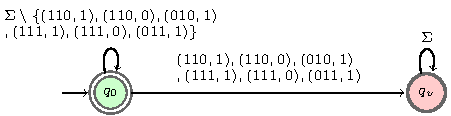
\includegraphics[width=0.5\columnwidth]{fig/sa1-crop2.pdf}
	}
	%	\hspace{0.1em}
	%	\subfloat[Input SA obtained from $\calA_{S_1}$. \label{fig:prop1Inp}]{
		%		\includegraphics[width=0.65\columnwidth]{figures/propA1I.png}
		%	}
	%	\\
	\centering
	\subfloat[SA $\calA_{S_2}$. \label{fig:prop2C}]{
		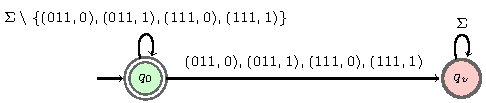
\includegraphics[width=0.5\columnwidth]{fig/sa2-crop2.pdf}
	}
	\hspace{0.1em}
	%	\subfloat[Input SA obtained from $\calA_{S_2}$. \label{fig:prop2Inp}]{
		%		\includegraphics[width=0.65\columnwidth]{figures/propA2I.png}
		%	}
	\caption{Safety automaton for $S_1$ and $S_2$.}
	\label{fig:prop1&2}
\end{figure*}
%%%%%%%%%%%%%%%%%%%%%%%%%%%%%
%%%%%%%%%%%%%%%%%%%%%%%%%%%%%%%%%%%%%%%%%%
\begin{example}[Example policies]
	\label{eg:propC}
	%%%%%%%%%%%%%%%%%%%%%%%%%%%%%%%%%%%%%%%%%%
	%In this section, we will consider the following properties:
	Let $I= \{A,B,C\}$ and $O = \{R\}$.
	Consider the following policies: \textit{$S_1$: ``A and B cannot happen simultaneously, and also B and R cannot happen simultaneously''} and \textit{$S_2$: ``B and C cannot happen simultaneously''}.
	The safety automaton in Figure~\ref{fig:prop1C} and Figure~\ref{fig:prop2C} define policies $S_1$ and $S_2$ respectively.
	%The input safety automaton in Figure~\ref{fig:prop1Inp} and %Figure~\ref{fig:prop2Inp} presents the input SA for $S_1$ and $S_2$ respectively.
\end{example}
%%%%%%%%%%%%%%%%%%%%%%%%%%%%%%%%%%%%%%%%%%%%%
%
%%%%%%%%%%%%%%%%%%%%%%%%%%%%%%%%%%%%%%%%%%%%%
\subsection{Monolithic security enforcement}
%%%%%%%%%%%%%%%%%%%%%%%%%%%%%%%%%%%%%%%%%%%%%
Composing all of the policies first is one way to enforce a collection of policies (taking the product of all the SA).
We can synthesize one enforcer for the resulting policy if the resulting SA is enforceable according to Definition~\ref{def:Enforceability}.


In the monolithic approach, policies (specified as SA) are first combined using intersection (see the Definition~\ref{def:product}, the product of SA), and an enforcer for the resulting policy is synthesized. Specifically, given any two
safety policies $\varphi_1$ and $\varphi_2$, to enforce both these policies, we first compute $\varphi =
\varphi_1 \cap \varphi_2$ (by computing the product of SA for $\varphi_1$ and $\varphi_2$). Then if the resulting SA for $\varphi$ is enforceable as per Definition \ref{def:Enforceability}, we synthesize
an enforcer for $\varphi$ using the approach described in Section \ref{sec:func:def}. 
%For any input word $\sigma$, $E_\varphi(\sigma)$ 
%is sound and transparent with respect to $\varphi_1 \cap \varphi_2$.

%%%%%%%%%%%%%%%%%%%%%%%%%%%%%%%%%%%%%%%%%%%
\begin{figure}[htb]
	\centering
	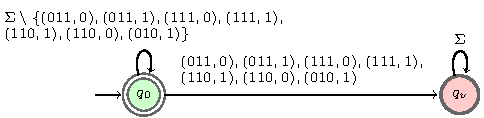
\includegraphics[scale=1]{fig/sa1sa2-crop2.pdf}
	\caption{$\calA_{S_1\cap S_2}$: Product of Automaton $S_1$ and $S_2$}
	\label{fig:prod}
\end{figure}
%%%%%%%%%%%%%%%%%%%%%%%%%%%%%%%%%%%%%%%%%%%

%%%%%%%%%%%%%%%%%%%%%%%%%%%%%%%%%%%%%%%%%%%%% 
\begin{example}[Monolithic approach]
	Consider policies $S_1$ and $S_2$ defined as SAs illustrated in Figure \ref{fig:prop1&2}.
	The SA obtained by taking the product of both these automata is shown in Figure \ref{fig:prod} defining the policy $S_1 \cap S_2$.
	The policy $S_1 \cap S_2$ is enforceable since for every accepting state, there is at least one outgoing transition to an accepting state (See Remark \ref{rem:nonEnf}). Table \ref{table:EgEnf} illustrates behavior of enforcer for policy $\calA_{S_1 \cap S_2}$ when the input-output word $(100,1)\cdot(110,1)\cdot(011,0)$ is processed incrementally.
\end{example}	
%%%%%%%%%%%%%%%%%%%%%%%%%%%%%%%%%%%%%%%%%%%%%

%%%%%%%%%%%%%%%%%%%%%%%%%%%%%%%%%%%
%
\begin{table}[t]
	\centering
	\scalebox{0.8}
	{
		\begin{tabular}{|c|c|c|c|}
			\hline
			$\sigma_I$ & $\sigma_O$ & $\efi(\sigma_I)$ & $\ef(\sigma)=\efo(\efi(\sigma_I), \sigma_O)$ \\
			\hline%
			$\epsilon_I$ & $\epsilon_O$ & $\epsilon_I$ & $(\epsilon_I,\epsilon_O) = \epsilon$\\
			\hline
			$100$ & $1$ & $100$ & $(100,1)$ \\
			\hline
			$100\cdot110$ & $1\cdot1$ & $100\cdot100$ & $(100,1)\cdot(100,1)$ \\
			\hline
			$100\cdot110\cdot011$ & $1\cdot1 \cdot0$ & $100\cdot 100 \cdot 001$ & $(100,1)\cdot(100,1) \cdot(001,0)$ \\
			
			\hline
		\end{tabular}
	}
	\caption{Example illustrating behavior of enforcer for $\calA_{S_1 \cap S_2}$}
	\label{table:EgEnf}
\end{table}
%%%%%%%%%%%%%%%%%%%%%%%%%%%%%%%%


%%%%%%%%%%%%%%%%%%%%%%%%%%%%%%%%%%%%%%%%%%%%% 
\begin{theorem}[Enforceability using the monolithic approach]
	\label{theorem:enforceability-monolithic}
	Consider two policies $\varphi_1$, $\varphi_2$ defined as SA, and $\varphi = \varphi_1 \cap \varphi_2$.
	
	If policy $\varphi_1$  or policy $\varphi_2$ is non-enforceable, then $\varphi_1 \cap \varphi_2$ is non-enforceable.
	%
	
	The proof of Theorem \ref{theorem:enforceability-monolithic} is given in Appendix \ref{proof:enforceability-monolithic}.
	%
	%\SP{We may have to add a brief justification/reasoning for the same.} \Abhinandan{kindly check}
	%This is very much intuitive. If $\varphi_1$  or property $\varphi_2$ is non-enforceable, then there would be no path to an accepting location from a designated location in the SA for any input event. As a result, as per the Definition \ref{def:product}, the product SA will contain a transition that will lead to violating state for any input. Then $\varphi_1 \cap \varphi_2$ is non-enforceable.
\end{theorem}	
%%%%%%%%%%%%%%%%%%%%%%%%%%%%%%%%%%%%%%%%%%%%% 

%%%%%%%%%%%%%%%%%%%%%%%%%%%%%%%%%%%%%%%%%%%%% 
\begin{remark}[Enforceability using the monolithic approach]
	Though policies $\varphi_1$ and $\varphi_2$ are enforceable individually, policy $\varphi_1 \cap \varphi_2$ may not be enforceable, as illustrated in the following example.
\end{remark}
%%%%%%%%%%%%%%%%%%%%%%%%%%%%%%%%%%%%%%%%%%%%% 


%%%%%%%%%%%%%%%%%%%%%%%%%%%%%
\ignore{
	\begin{figure*}
		\begin{centering}
			\scalebox{0.9}{
				\includegraphics[scale=0.1]{fig/nonEnf1.jpg}
			}
			\caption{Policy $\varphi_1\cap \varphi_2$ is non-enforceable. \SP{Abhinandan, you may pl work on this fig and the corresponding explanation of the example!}}
			\label{fig:nonEnf1}
		\end{centering}
	\end{figure*}
} 
%%%%%%%%%%%%%%%%%%%%%%%%%%%%%
%%%%%%%%%%%%%%%%%%%%%%%%%%%%%%%%%%%%%%%%%%%%% 


%%%%%%%%%%%%%%%%%%%%%%%%%%%%%
\begin{figure}%
	\centering
	
	
	\subfloat[SA defining $\varphi_1$- Enforceable \protect\footnotemark]{{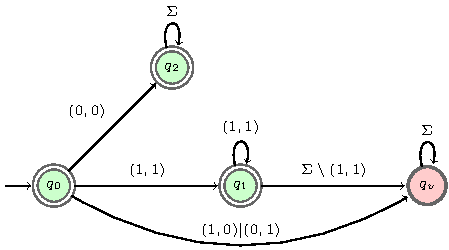
\includegraphics[]{fig/Phi1-crop2.pdf} }}%
	%\qquad
	\vspace{2em}
	\subfloat[SA defining $\varphi_2$- Enforceable \protect\footnotemark ]{{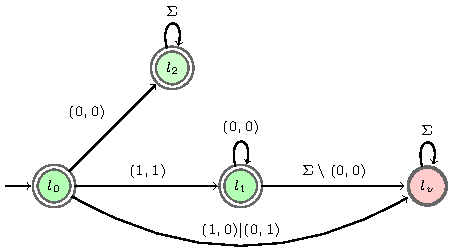
\includegraphics[]{fig/Phi2-crop2.pdf} }}%
	%\qquad
	\vspace{2em}
	\subfloat[SA defining $\varphi_1$ $\cap$ $\varphi_2$]{{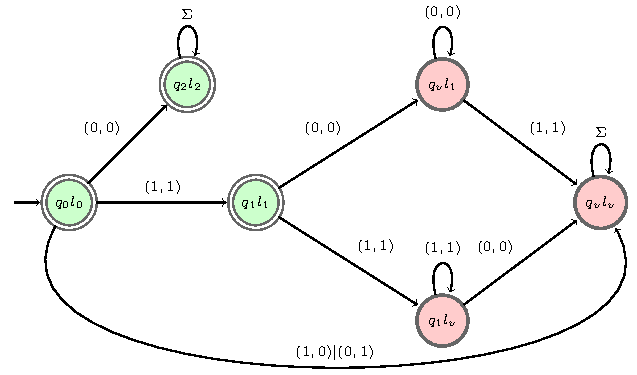
\includegraphics[width=0.9\columnwidth]{fig/Phi1-and-Phi2-cropped.pdf} }}%	
	\caption{Policy $\varphi_1\cap \varphi_2$ is non-enforceable.}
	%	\SP{TO follow a particular color conventions. Reduce space!}
	\label{fig:nonEnf1}
	\vspace{2em}
\end{figure}
\footnotetext[2]{Here, $\Sigma = \{(0,0), (0,1), (1,0), (1,1)\}$. So $\Sigma \setminus (1,1) $ = $\{(0,0), (0,1), (1,0)\}$.}
\footnotetext[3]{Here, $\Sigma = \{(0,0), (0,1), (1,0), (1,1)\}$. So $\Sigma \setminus (0,0) $ = $\{ (0,1), (1,0), (1,1)\}$.}
%%%%%%%%%%%%%%%%%%%%%%%%%%%%%%%%%%%%%%%%%%%%%%%%%%%%%%%%%%%%%%%
\begin{example}[Monolithic approach does not always work]
	Consider the two policies shown in Figure \ref{fig:nonEnf1}. Here $I= \{0,1\}$ and $O = \{ 0,1 \}$. Though they are enforceable individually, the policy that we obtain by taking the product of both the SA $\varphi_1 \cap \varphi_2$ is not enforceable. 
	Suppose that the first event is $(1,1)$, the output of the enforcer will be $(1,1)$, and the state of the product automaton will be updated to $(q_1,l_1)$. When in state $(q_1,l_1)$, whatever may be the input event, it is not possible to correct it (as there will be no path to an accepting state from the state $(q_1,l_1)$ in the product automaton). 
\end{example}	
%%%%%%%%%%%%%%%%%%%%%%%%%%%%%%%%%%%%%%%%%%%%%%%%%%%%%%%%%%%%%%%%%%%%%%%%%%%%%%%%%%%%%%%%%% 
\ignore{
	In \cite{cre2017}, serial and parallel composition approaches were presented. It is shown in \cite{cre2017} that both the compositional approaches work if all the policies are prefix-closed safety policies. However, the enforcement approach considered in \cite{cre2017} is not suitable for reactive systems, since it allows only delaying of events.   }

%In our framework, though prefix-closed safety policies are considered, since the framework allows editing of events, and since enforcers are bi-directional, it is not possible to compose enforcers (as per Definition \ref{def-func-E}) in series or in parallel for the following reasons: 
As discussed in the problem description in the introduction, we focus on how to add a new enforcement layer incrementally to the existing enforcer (e.g., when a new property to be enforced is identified due to a new threat). 
How can an enforcer for the new property be composed with an existing enforcer such that the composed enforcement system, along with the new policy\blue{,} will also continue to enforce all the previously enforced policies is what we explore and study in this work.   



In our framework, since the framework allows editing of events, and since enforcers are bi-directional, it is not possible to compose enforcers (as per Definition \ref{def-func-E}) for the following reasons: 

\squishlist
\item As illustrated in Figure \ref{fig:intro-context}, the enforcer is bi-directional. Firstly, input from the environment is read (and edited/corrected if necessary), which is fed to the program, and the resulting output of the program is later checked (and edited if necessary) by the enforcer before it is forwarded to the environment. This does not allow the enforcers that we have to be composed directly in series. 
\item Moreover, since editing of events is allowed, the edit/correction made by one enforcer may not be compatible w.r.t the other enforcer, where there may be some edit/correction that is suitable for both policies to be enforced.  
\squishend
%%%%%%%%%%%%%%%%%%%%%%%%%%%%%%%%%%%%%%%%%%%%%%%%%%%%%%%%%%%%%%%%%%%%%%%%%%%%%%%%%%%%%%%%%%

Thus we need to revisit the definition of the enforcement function, which will also be suitable for incremental enforcement schemes.
%%%%%%%%%%%%%%%%%%%%%%%%%%%%%%%%%%%%%%%%%%%%%%%
\subsection{Incremental composition of security enforcers} 
\label{sec:serial}
%%%%%%%%%%%%%%%%%%%%%%%%%%%%%%%%%%%%%%%%%%%%%%
Suppose that we rely on the internals of the enforcement function, which composes an input enforcement function and an output enforcement function, then we can consider:
%in serial composition approach,
\squishlist
\item composing all the input enforcement functions in series, where the (corrected) input that is released by the last function is fed to the program.
\item similarly, the output enforcement functions can also be combined in series\blue{,} and the corrected output released by the last function can be emitted to the environment. 
\squishend

The incremental scheme by composing enforcers in series is shown in Figure \ref{fig:serialComp1}.

%%%%%
%\SP{Abhinandan, may pl add a figure illustrating the scheme/approach.}
%%%%%%%%%%%%%%%%%%%%%%%%%%%%%%%%%%%%
Given two policies $\varphi_1$ and $\varphi_2$ (where $\varphi_{1I}$ and $\varphi_{2I}$ are their corresponding input policies)\blue{,} we can synthesize input and output enforcement functions for each of these policies $\efi{\varphi_1}$,  $\efi{\varphi_2}$, $\efo{\varphi_1}$, and $\efo{\varphi_2}$, 
and then compose all the input enforcers and all the output enforcers. The composed input enforcer can be then combined with the composed output enforcer (see Figure \ref{fig:serialComp1}).

%%%%%%%%%%%%%%%%%%%%%%%%%%%%%%%%%%%%%%%%%%%%%%%
\begin{SingleColFigure}
	\centering
	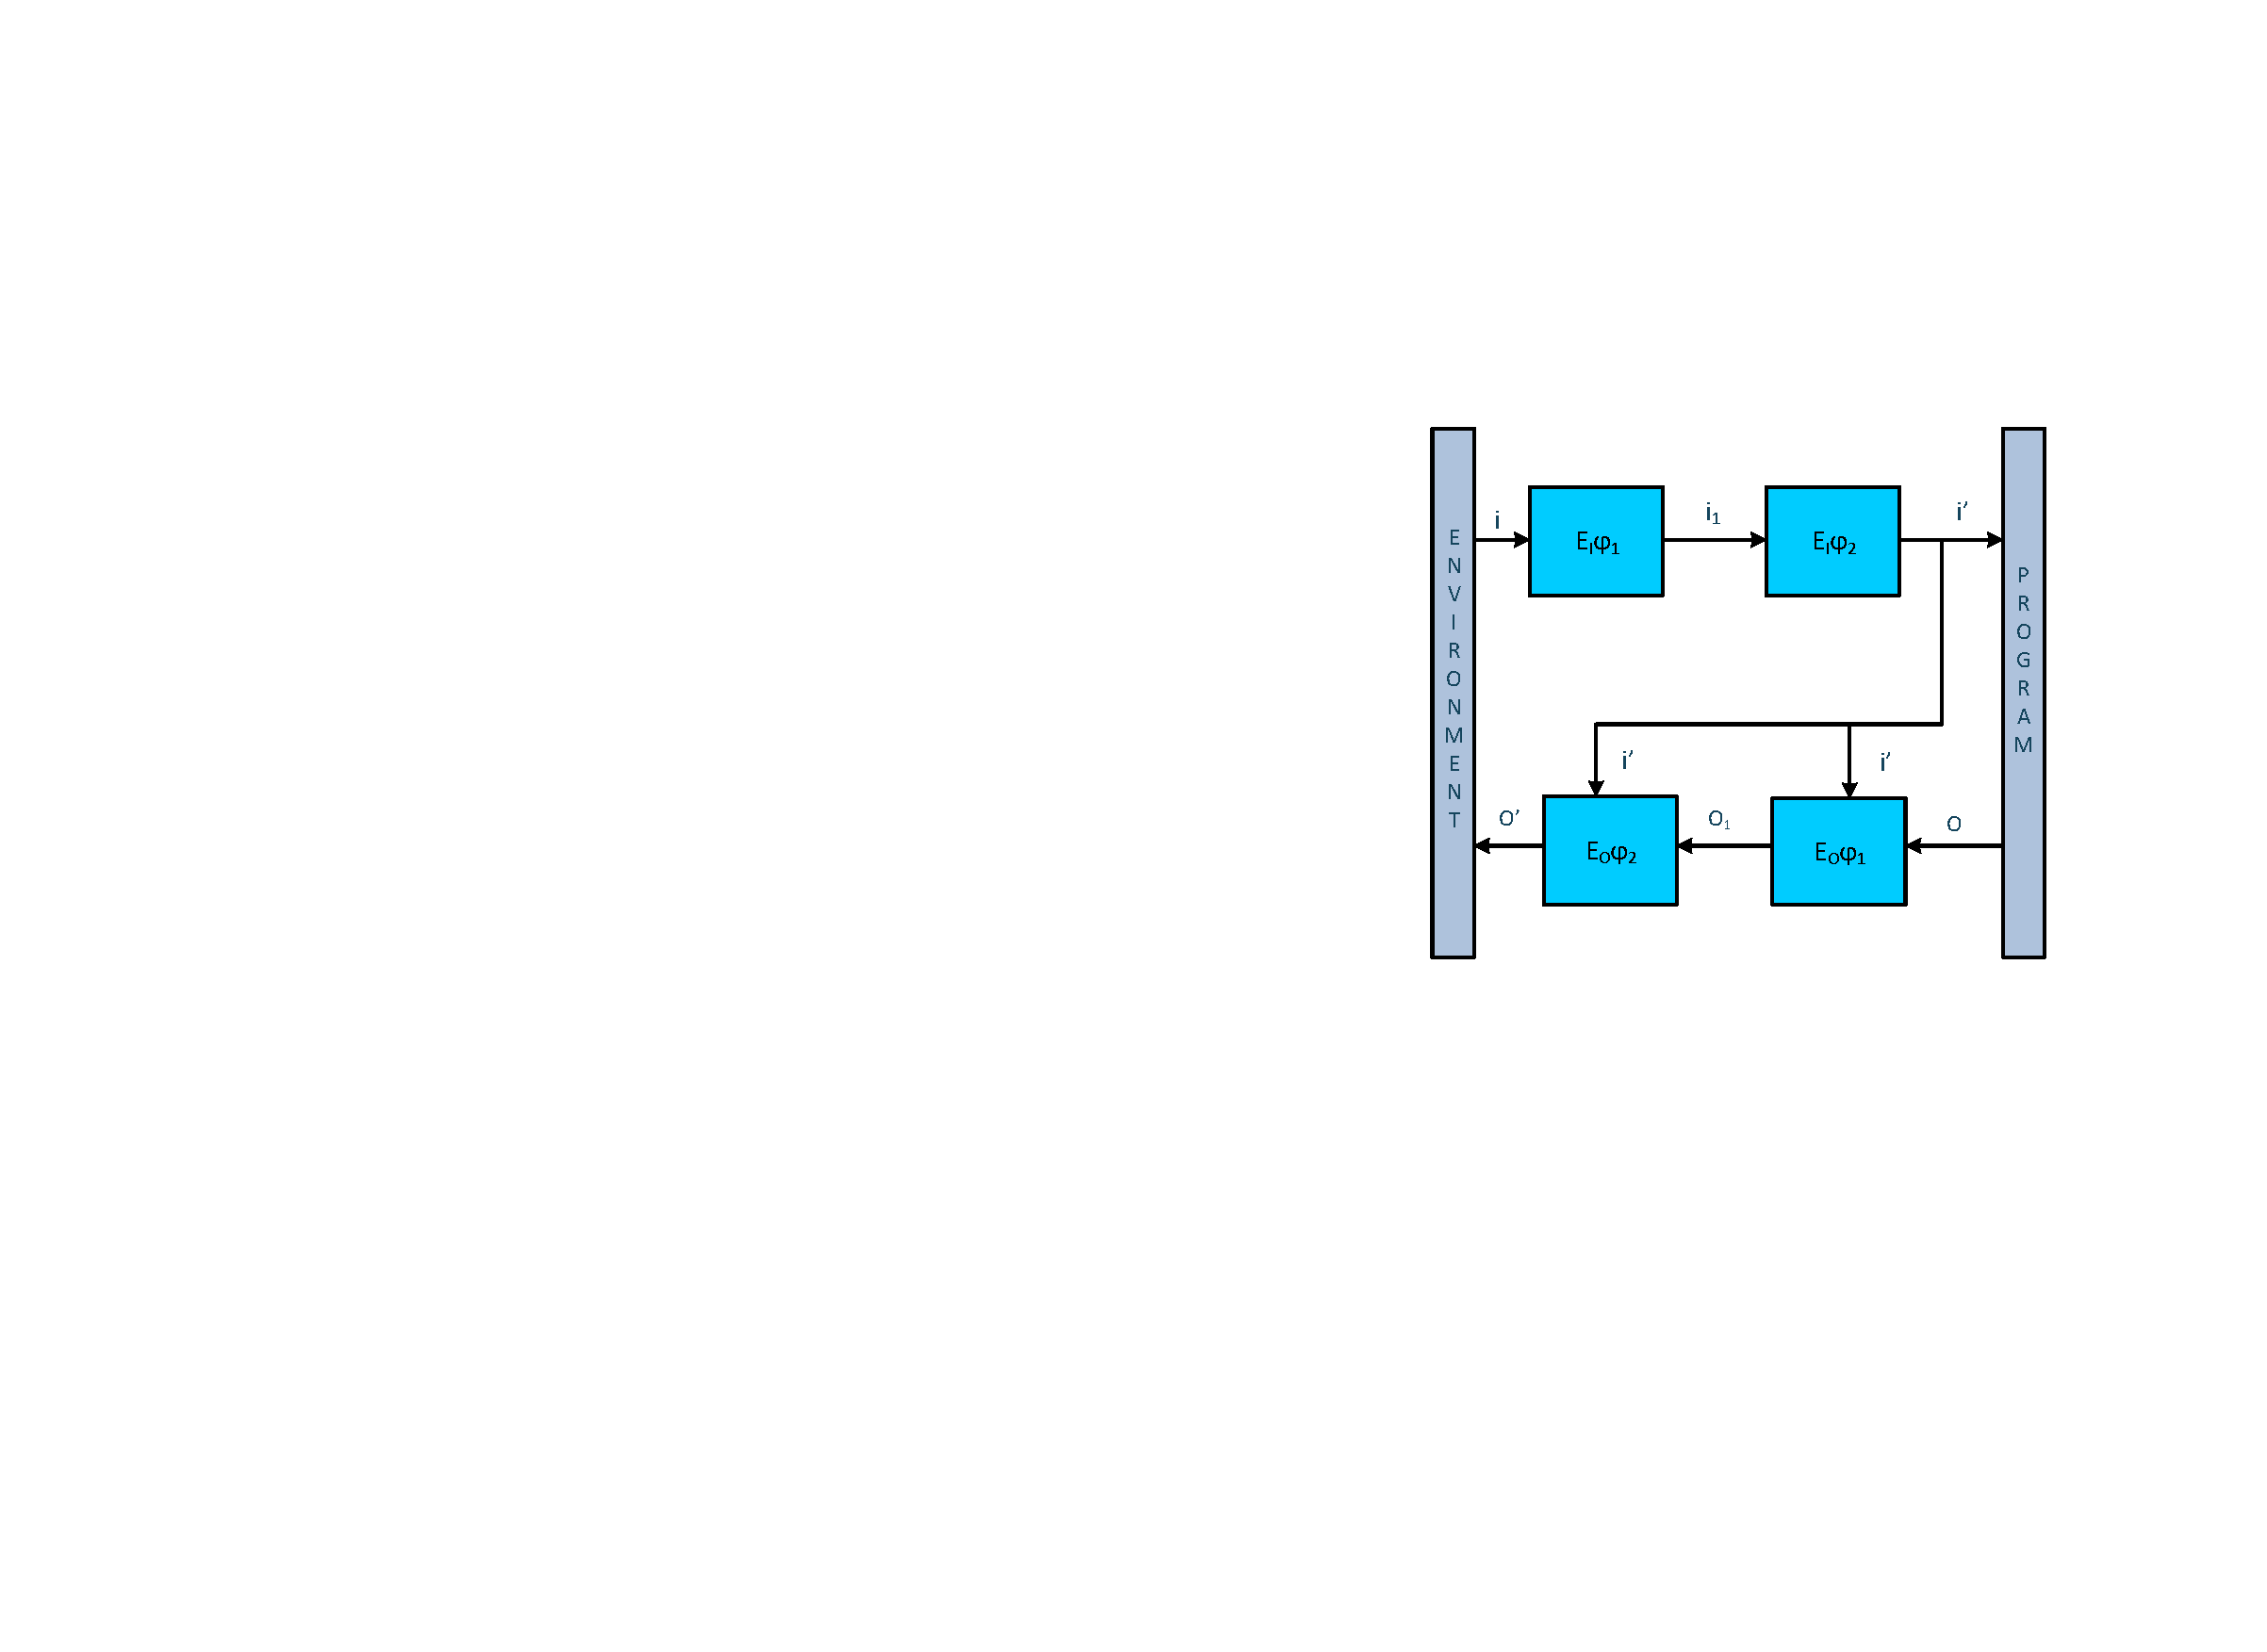
\includegraphics[width=\columnwidth]{fig/serial composition-ColourDiagram-cropped2.pdf}
	\captionof{figure}{Incremental enforcement via serial composition}
	%\SP{Abhinandan, may pl add a figure !}
	
	\label{fig:serialComp1}
\end{SingleColFigure}
%%%%%%%%%%%%%%%%%%%%%%%%%%%%%%%%%%%%%%%%%%

We denote this type of incremental composition of enforcers in series as  $\e{\varphi_1} \serial \e{\varphi_2}$.
% In this type of serial composition, the output of $\e{\varphi_1}$ is fed as input to $\e{\varphi_2}$. As a result we obtain a new EM, denoted $\e{\varphi_1} \serial \e{\varphi_2}$.
In this section we investigate whether $\e{\varphi_1} \serial \e{\varphi_2}$
generally enforces $\varphi_1\cap\varphi_2$.
We are also interested to see whether the final output that we obtain using the incremental composition approach is equal to the output we would obtain using the monolithic approach.
%%%%%%%%%%%%%%%%%%%%%%%%%%%%%%%%%%%%%

Let us now formally define incremental composition in series of two enforcers.

%%%%%%%%%%%%%%%%%%%%%%%%%%%%%%%%%%
\begin{definition}[Incremental enforcement via serial composition]
	\label{def:serialComp}
	Let $\efi{\varphi_1}: \Sigma_I^* \rightarrow \Sigma_I^*$ (resp. $\efi{\varphi_2}: \Sigma_I^* \rightarrow \Sigma_I^*$) be the input enforcement function for policy $\varphi_{1I}  \subseteq \Sigma_I^*$ (resp. $\varphi_{2I}$), and 
	let 
	$\efo{\varphi_1}: \Sigma_I^* \times \Sigma_O^* \rightarrow (\Sigma_I \times \Sigma_O)^*$ (resp. $\efo{\varphi_2}$) be the output enforcement function for policy $\varphi_1  \subseteq \Sigma^*$ (resp. $\varphi_2$). 
	Their serial composition is a new enforcer $\e{\varphi_1} \serial \e{\varphi_2}: \Sigma^* \rightarrow \Sigma^*$ defined as follows:
	\[
	\forall \sigma\in\Sigma^*,
	(\e{\varphi_1} \serial \e{\varphi_2})(\sigma)
	= \efo{\varphi_2}(\sigma'_I, \sigma'_O).
	\]
	with $\sigma'_I = \efi{\varphi_2}(\efi{\varphi_1}({\sigma_I}))$, and $\sigma'_O = \efo{\varphi_1}(\sigma'_I, \sigma_O)$.
\end{definition}
%%%%%%%%%%%%%%%%%%%%%%%%%%%%%%%%%%
%%%%%%%%%%%%%%%%%%%%%%%%%%%%%%%%%%
%\SP{We may add a brief 1-2 lines expl of the def.}\Abhinandan{kindly check.}
As per the composition Definition \ref{def:serialComp}, the output of the serial composition of the enforcers is the output emitted from the output enforcer \efo{$\varphi_2$}. The input emitted from the input enforcer \efi{$\varphi_2$} is considered as the final corrected input. The output enforcer \efo{$\varphi_1$} is invoked with the corrected input $\sigma'_I$ from the serially composed input enforcers and the output $\sigma_O$ of the reactive system. The corrected output of the enforcer is input to the output enforcer \efo{$\varphi_2$}, which finally emits the output to the environment.   
%%%%%%%%%%%%%%%%%%%%%%%%%%%%%%%%%%%%%

\begin{table*}
	%\vspace{-1em}
	\centering
	\begin{tabular}{|c|c|c|c|c|c|}
		\hline
		$\sigma_I$ & $\sigma_O$ & $\sigma'_I = \efi{S1}(\sigma_I)$ & $\sigma^{''}_I = \efi{S2}(\sigma'_I)$ & $ \sigma'_O = \efo{S1}(\sigma^{''}_I, \sigma_O)$ & $\efo{S2}(\sigma^{''}_I, \sigma'_O)$ \\
		\hline
		$100$ & $1$ & $100$ & $100$ &  $(100,1)$ & $(100,1)$ \\
		\hline
		$100 \cdot 110$ & $1 \cdot 1 $ & $100 \cdot 011$ & $100 \cdot 110$ &  $(100,1) \cdot ??$ & -- \\
		
		\hline
	\end{tabular}
	\caption{Serial composition using Definition \ref{def:serialComp}}
	\label{tableEgSerialDef}
\end{table*}
%%%%%%%%%%%%%%%%%%%%%%%%%%%%%%%%%%%%%%%%%%%%%%%%%%%%%%%%%%%%%%%%%%%%%%%%%
\begin{figure*}
	%
	\centering
	\subfloat[SA $\calA_{S_1}$. \label{fig:prop1C}]{
		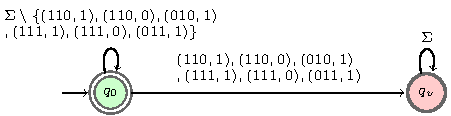
\includegraphics[width=0.5\columnwidth]{fig/sa1-crop2.pdf}
	}
	%	\hspace{0.1em}
	%	\subfloat[Input SA obtained from $\calA_{S_1}$. \label{fig:prop1Inp}]{
		%		\includegraphics[width=0.65\columnwidth]{figures/propA1I.png}
		%	}
	%	\\
	\centering
	\subfloat[SA $\calA_{S_2}$. \label{fig:prop2C}]{
		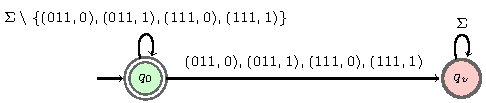
\includegraphics[width=0.5\columnwidth]{fig/sa2-crop2.pdf}
	}
	\hspace{0.1em}
	%	\subfloat[Input SA obtained from $\calA_{S_2}$. \label{fig:prop2Inp}]{
		%		\includegraphics[width=0.65\columnwidth]{figures/propA2I.png}
		%	}
	\caption{Safety automaton for $S_1$ and $S_2$.}
	\label{fig:prop1&2-duplicate}
\end{figure*}
%%%%%%%%%%%%%%%%%%%%%%%%%%%%%%%%%%%%%%%%%%%%%%%%%%%%%%%%%%%%%%%%%%%%%%%%%%%%%%%%%%%%%%%%%%%%%%%%%%%%
\begin{remark}
	
	Definition \ref{def:serialComp} is formulated in order to support incrementally adding a new enforcement layer. Suppose that we only have the input and output enforcement functions w.r.t policy $\varphi_1$ and a new policy to be enforced $\varphi_2$ is given. 
	We can obtain enforcement functions for $\varphi_2$ individually and compose with the existing enforcement functions as per Definition \ref{def:serialComp}.
	
\end{remark}
%%%%%%%%%%%%%%%%%%%%%%%%%%%%%%%%%%%%%

\emph{Note that serial composition of enforcers as per Definition \ref{def:serialComp} does not always work. 
	That is, though given two policies $\varphi_1$, $\varphi_2$ and also $\varphi_1 \cap \varphi_2$ are all enforceable, the serial composition of enforcers of $\varphi_1$ and $\varphi_2$ as per the above definition may not work. The final output obtained may not satisfy $\varphi_1 \cap \varphi_2$. Moreover, there may also be situations where other constraints\blue{,} such as instantaneity\blue{,} may be violated.} Let us consider input enforcement to understand this (similar reasoning also applies for output enforcement). As per the serial composition definition (Def. \ref{def:serialComp}), the input emitted from the input enforcer \efi{$\varphi_2$} is considered as the final corrected input, but the final input selected by the function $\efi{\varphi_2}$  may violate the policy monitored by the input enforcer $\efi{\varphi_1}$.     

Let us consider the following example to understand this further.


\begin{example}[{Serial composition as per Definition \ref{def:serialComp} does not always work}]
	Let us again consider policies $S_1$ and $S_2$ illustrated in Figure \ref{fig:prop1&2}, presented again in Figure \ref{fig:prop1&2-duplicate}. 
	Both policies $S_1$ and $S_2$ are enforceable individually. The policy $S_1 \cap S_2$ is also enforceable. 
	However, when we compose input and output enforcers for these policies in series as per Definition \ref{def:serialComp}, the final output obtained may not satisfy policy $S_1 \cap S_2$. 
	Also, there may be situations where constraints such as instantaneity may be violated. 
	For example\blue{,} consider the word $(100,1) \cdot (110,1) \cdot (011,0)$ to be processed incrementally.   
	In the first step, $(100,1)$ satisfies both policies and thus will be emitted as it is.
	In the second step, let us consider that the altered input produced by the second input enforcement function is $110$. 
	When $110$ is fed as input to the output enforcement function of policy $S_1$, there is no possible output event that it can release to satisfy policy $S_1$. The incremental processing of the considered word is shown in Table \ref{tableEgSerialDef}.	
\end{example}

%%%%%%%%%%%%%%%%%%%%%%%%%%%%%%%%%%
%%%%%%%%%%%%%%%%%%%%%%%%%%%%%%%%%%%
\ignore{
	\begin{table*}
		\vspace{-1em}
		\centering
		\begin{tabular}{|c|c|c|c|c|c|}
			\hline
			$\sigma_I$ & $\sigma_O$ & $\sigma'_I = \efi{S1}(\sigma_I)$ & $\sigma^{''}_I = \efi{S2}(\sigma'_I)$ & $ \sigma'_O = \efo{S1}(\sigma^{''}_I, \sigma_O)$ & $\efo{S2}(\sigma^{''}_I, \sigma'_O)$ \\
			\hline
			$100$ & $1$ & $100$ & $100$ &  $(100,1)$ & $(100,1)$ \\
			\hline
			$100 \cdot 110$ & $1 \cdot 1 $ & $100 \cdot 011$ & $100 \cdot 110$ &  $(100,1) \cdot ??$ & -- \\
			
			\hline
		\end{tabular}
		\caption{Serial composition using definition \ref{def:serialComp}}
		\label{tableEgSerialDef}
	\end{table*}
}
%%%%%%%%%%%%%%%%%%%%%%%%%%%%%%%%
%%%%%%%%%%%%%%%%%%%%%%%%%%%%%%%%
%
%%%%%%%%%%%%%%%%%%%%%%%%%%%%%%%%%%%%%%%%%%%%%%%%
%\subsection{Parallel composition of enforcers} 
%\label{sec:parallel}
%%%%%%%%%%%%%%%%%%%%%%%%%%%%%%%%%%%%%%%%%%%%%%%
%
%
%Parallel composition of enforcers generally does not work because enforcers should react instantaneously and they are allowed to edit events.
%%%%%%%%%%%%%%%%%%%%%%%%%%%%%%%%%%%%%%%%%%%%%%%%
%\begin{SingleColFigure}
%	\centering
%	\includegraphics[width=0.9\columnwidth]{figures/parallel1.jpeg}
%	\captionof{figure}{Parallel Composition \SP{Abhinandan, may pl add a figure !}}
%	\label{fig:parallelComp1}
%\end{SingleColFigure}
%%%%%%%%%%%%%%%%%%%%%%%%%%%%%%%%%%%%%%%%%%%%%%%%
%%%%%%%%%%%%%%%%%%%%%%%%%%%%%%%%%%%%%%%%%%%%%%%%
%\begin{SingleColFigure}
%	\centering
%	\includegraphics[width=0.9\columnwidth]{fig/parallel-composition-crop.pdf}
%	\captionof{figure}{Parallel Composition}
%	\label{fig:parallelComp1}
%\end{SingleColFigure}
%%%%%%%%%%%%%%%%%%%%%%%%%%%%%%%%%%%%%%%%%%%%%%%%
%\vspace{0.5em}
%Let us consider parallel composition of the input enforcers. At the beginning of each tick, each input enforcer is fed with the same input (input observed from the environment), each of them emits a corrected input according to its property. There should be some mechanism for selecting one corrected input from the corrected inputs emitted by all the enforcers. 
%
%Let us consider two properties $\varphi_1$ and $\varphi2$ (where $\varphi_{1I}$ and $\varphi_{2I}$ are their corresponding input properties). we can synthesize input and output enforcement functions for each of these properties $\efi{\varphi_1}$,  $\efi{\varphi_2}$, $\efo{\varphi_1}$, and $\efo{\varphi_2}$.
% 
%As illustrated in Figure \ref{fig:parallelComp1}, we can consider composing the input enforcers in parallel, where input from the environment $i$ is fed as input to both the input enforcers in parallel. Each input enforcer emits transformed input $i_1$ (resp. $i_2$), which are fed as input to the $Merge_I$ function, which picks one among them randomly ($i'$) and emits it to the program. 
%
%Similarly, the output from the program $o$ can be fed in parallel to both the output enforcers  $\efo{\varphi_1}$, and $\efo{\varphi_2}$, Each output enforcer produces transformed output $o_1$ (resp. $o_2$). which are fed as input to the $Merge_O$ function, which picks one among them randomly ($o'$) and emits it to the environment. 
%   
%
%%%%%%%%%%%%%%%%%%%%%%%%%%%%%%%%%%%%%%%%%%%%%%%%%%%%%%%%%%%%%%%%%
%%%%%%%%%%%%%%%%%
%\begin{definition}[Parallel composition of enforcement monitors]
%	\label{def:parallelComp}
%Let $\efi{\varphi_1}: \Sigma_I^* \rightarrow \Sigma_I^*$ (resp. $\efi{\varphi_2}: \Sigma_I^* \rightarrow \Sigma_I^*$) be the input enforcement function for property $\varphi_{1I}  \subseteq \Sigma_I^*$ (resp. $\varphi_{2I}$), and 
%let 
%$\efo{\varphi_1}: \Sigma_I^* \times \Sigma_O^* \rightarrow (\Sigma_I \times \Sigma_O)^*$ (resp. $\efo{\varphi_2}$) be the output enforcement function for property $\varphi_1  \subseteq \Sigma^*$ (resp. $\varphi_2$). 
%
%Their parallel composition is a new enforcer $\e{\varphi_1} || \e{\varphi_2}: \Sigma^* \rightarrow \Sigma^*$ defined as follows:
%
%	$
%	\forall \sigma\in\Sigma^*, (\e{\varphi_1}|| \e{\varphi_2})(\sigma) = Merge_O(\efo{\varphi_1}(\sigma'_I, \sigma_O), \efo{\varphi_2}(\sigma'_I, \sigma_O)).
%	$
%	
%	with $\sigma'_I = Merge_I(\efi{\varphi_1}(\sigma_I), \efi{\varphi_2}(\sigma_I))$.
%\end{definition}
%%%%%%%%%%%%%%%%%%%%%%%%%%%%%%%%%%%%%%%%%%%%%%%%%%%%%%%%%%%%%%%%
%
%
%%There is no such possible mechanism, as selecting any input from the corrected inputs emitted the input enforcers may violate the property monitored by the other input enforcers. 
%
%
%Note that parallel composition of enforcers does not always work. That is, though given two properties $\varphi_1$, $\varphi_2$ and also $\varphi_1 \cap \varphi_2$ are all enforceable, parallel composition of enforcers of $\varphi_1$ and $\varphi_2$ as per the above definition may not work. The final output obtained may not satisfy $\varphi_1 \cap \varphi_2$. Moreover, there may be also situations where other constraints such as instantainety may be violated.
%Let us consider input enforcement to understand this (similar reasoning also applies for output enforcement). As per the parallel composition definition (Def. \ref{def:parallelComp}), any input from the corrected inputs emitted the input enforcers can be selected as the final corrected input. The final input selected by the $Merge_I$ function may violate the property monitored by the some of the input enforcers.     
%
%Let us consider the following example to understand this further.
%
%%%%%%%%%%%%%%%%%%%%%%%%%%%%%%%%%%%
%%%%%%%%%%%%%%%%%%%%%%%%%%%%%%%%%%%%
%%
%\begin{table*}[]
%	\centering
%	\begin{tabular}{|c|c|c|c|c|c|c|c|}
	%		\hline
	%		$\sigma_I$ & $\sigma_O$ & $\efi{S1}(\sigma_I)$ & $\efi{S2}(\sigma_I)$ & $\sigma'_I= Merge_I()$ & $\efo{S1}(\sigma'_I, \sigma_O)$&$\efo{S2}(\sigma'_I, \sigma_O)$&$Merge_O()$\\
	%		\hline
	%		$100$ & $1$ & $100$ & $100$ & $100$& $(100,1)$ & $(100,1)$ & $(100,1)$ \\
	%		\hline
	%		$100 \cdot 110$ & $1 \cdot 1 $ & $100 \cdot 011$ & $100 \cdot 110$& $100 \cdot 110$ & $(100,1) \cdot ?? $ & -- & -- \\
	%%		
	%		\hline
	%	\end{tabular}
%	\caption{Parallel composition}
%	\label{tableEgParallelDef}
%\end{table*}
%%%%%%%%%%%%%%%%%%%%%%%%%%%%%%%%%
%%%%%%%%%%%%%%%%%%%%%%%%%%%%%%%%%
%\begin{example}[Parallel composition does not work]
%
%Let us again consider properties $S_1$ and $S_2$ illustrated in Figure \ref{fig:prop1&2}. 
%Both properties $S_1$ and $S_2$ are enforceable individually. The property $S_1 \cap S_2$ is also enforceable. 
%However, when we compose input and output enforcers for these properties in parallel as per Definition \ref{def:parallelComp}, the final output obtained may not satisfy property $S_1 \cap S_2$. %Also, there may be situations where constraints such as instantainety may be violated.
% For example consider the word $(100,1) \cdot (110,1) \cdot (011,0)$ to be processed incrementally.   
%In the second step, when the input $110$ is fed to both the input enforcement function parallely, the two enforcers may emit $011$ and $110$, respectively satisfying respective property. As per parallel composition mechanism, any one of the corrected inputs may be emmitted as the final output, say $110$ in this case. When the input given to the output enforcement function of property $S_1$ is $110$, there is no possible input-output event that it can release as output continuing to satisfy property $S_1$. The incremental processing of the considered word is shown in Table \ref{tableEgParallelDef}.	
%
%\SP{Abhinandan, may pl check, explain the example!}	
%\end{example}

%\blue{We thus revisit the incremental security enforcement scheme in the next section.   
	%}

In this section, we have seen that the enforcement function in Definition \ref{def-func-E}  is not always suitable for the incremental security enforcement by composing enforcers in series, also when we consider first composing all the input enforcement functions, followed by the composition of the output enforcement functions (Definition \ref{def:serialComp}).



We thus revisit the incremental security enforcement scheme in the next section, to propose an incremental scheme that can tackle all the enforceable properties.


%%%%%%%%%%%%%%%%%%%%%%%%%%%%%%%%%%%%%%%%%%%%%%%%%%%%%%%%
%%%%%%%%%%%%%%%%%%%%%%%%%%%%%%%%%%%%%%%%%%%%%%%%%%%%%%%%
\section{Revisiting Incremental Security Enforcement  Scheme}
\label{sec:new:def}
%(its corresponding enforcement algorithm given in Definition \ref{def:Enforceability})
In this section we propose an incremental composition scheme. First, we define the following Select functions and later present how the compositional scheme can be defined using the Select functions. 
%We later define serial and parallel composition and show that for any given set of properties, that are enforceable using the monolithic approach, they are also enforceable using both serial and parallel composition schemes.

%%%%%%%%%%%%%%%%%%%%%%%%%%%%%%%%%%%%%%%%%%%%%%%%%%%%%%%%
%%%%%%%%%%%%%%%%%%%%%%%%%%%%%%%%%%%%%%%%%%%%%%%%%%%%%%%% 
%
%%%%%%%%%%%%%%%%%%%%%%%%%%%%%%%%%%%%%%%%%%%%%%%%%%%%%%%%
\subsection{Select Functions}
\label{sec:new:edit}
%%%%%%%%%%%%%%%%%%%%%%%%%%%%%%%%%%%%%%%%%%%%%%%%%%%%%%%%
%\red{Briefly discuss why we need to redefine edit functions in the following manner. Set of all possible inputs fed to the first edit/select function.}

%\SP{Abhinandan, pl check the notes/presentation and see to revise these definitions !}
%

%\SP{We may add simple examples to illustrate these select functions.}\Abhinandan{kindly check.}
\squishlist
\item {{\boldmath$\selectI_{\varphi_{I}}(\sigma_I, X)$}}: Given an input word $\sigma_I\in\Sigma_I^*$, and a set of input events $X \subseteq \Sigma_I$, $\selectI_{\varphi_{I}}(\sigma_I, X)$ is the set of input events $x$ that belong to set $X$ such that the word obtained by extending $\sigma_I$ with $x$ satisfies policy $\varphi_I$. Formally,
\[\selectI_{\varphi_{I}}(\sigma_I, X) = \{ x\in X: \sigma_I \cdot x \models \varphi_I \}.\]
%
Considering the SA $\calA_{\varphi_I}=(Q, q_0, q_v, \Sigma_I, \rightarrow_I)$,
the set of events in $X$ that allow to reach a state in $Q\setminus \{q_v\}$ from a state $q\in Q\setminus \{q_v\}$ is defined as:
\[\selectI_{\calA_{\varphi_I}}(q,X) = \{x\in X: q \xrightarrow{x}_I q' \wedge q' \neq q_v \}. \]
%
For example, let us consider the input automaton corresponding to policy $P$ in Figure \ref{fig:prop1Inp}.
Initially, when $\sigma_I = \epsilon$ we have $X = \{00,01,10,11\}$, and $\selectI_{P}(\epsilon, X)= \{00,01,10\}$.
%
If we consider $\sigma_I = 00 \cdot 01 \cdot 01$, and  $X = \{00,01,10\}$, we have $\selectI_{P}(00 \cdot 01, X)= \{00,01,10\}$.

Also, $q_0 \xrightarrow{00\cdot01}_I q_0$, and $\selectI_{P}(q_0, \{00,01,10\}) = \{00,01,10\}$.


%For example, consider the the property $S_1$ illustrated in Figure \ref{fig:prop1&2} by ignoring outputs. In this case, the set of valid inputs, $X$= $(100,101,010,001,011)$. Let $\sigma= (100,1)\cdot(110,1)$, and thus $\sigma_I= 100\cdot110$. Then, $\selectI_{S1}(\sigma_I, X)=\{100,101,010,001,011\}$.

%$\editI(\sigma_I) = \Sigma_I\setminus\{11\}$.


%Also, $q_0 \xrightarrow{100\cdot110}_I q_0$, and $\selectI_{S1}(q_0,X) = \{100,101,010,001,011\}$.



%If $\editIaut(q)$ is non-empty, then $\randEditIaut(q)$ returns an element (chosen randomly) from $\editIaut(q)$, and is undefined if $\editIaut(q)$ is empty.
%
\item {\boldmath$\selectO_\varphi(\sigma, x, Y)$}:~~Given an input-output word $\sigma\in\Sigma^*$, an input event $x\in\Sigma_I$, and a set of output events $Y \subseteq \Sigma_O$, $\selectO_\varphi(\sigma, x, Y)$ is the set of output events $y$ in $Y$ s.t. the input-output word obtained by extending $\sigma$ with $(x,y)$ satisfies policy $\varphi$. Formally,
\[\selectO_\varphi(\sigma,x, Y) = \{y \in Y: \sigma \cdot (x,y) \models \varphi \}.\]
%
Considering the automaton $\calA_{\varphi}=(Q, q_0, q_v, \Sigma, \rightarrow)$ defining policy $\varphi$, and an input event $x\in\Sigma_I$,
the set of output events $y$ in $Y$ that allow to reach a state in $Q\setminus \{q_v\}$ from a state $q\in Q\setminus \{q_v\}$ with $(x,y)$ is defined as:
\[\selectO_{\calA_{\varphi}}(q,x, Y) = \{y \in Y: q \xrightarrow{(x,y)} q' \wedge q' \neq q_v \}. \]
%
\squishend

For example, consider policy $P$ illustrated in Figure \ref{fig:prop1}. We have $\selectO_{P}(q_0, 01, \{0,1\}) = \{0\}$.

%For example, consider property $S_1$ defined by the automaton in Figure~\ref{fig:prop1}.
%We have $\editOaut(q_0, 01) = \{0\}$.
%
%If $\editOaut(q,x)$ is non-empty, then $\randEditOaut(q, x)$ returns an element (chosen randomly) from $\editOaut(q,x)$, and is undefined if $\editOaut(q,x)$ is empty.




{\boldmath$\minEdit(x, X')$ (resp. \boldmath$\minEdit(y, Y')$)}: Consider $X'$ (resp. $Y'$) as a set of input (resp. output) events acceptable to all policies $\varphi$, and $x$ (resp. $y$) as the original input (resp. output). $\minEdit(x, X')$ (resp. $\minEdit(y, Y')$) non-deterministically selects an edit $x' \in X'$ (resp. $y' \in Y'$) such that it is of minimum deviation from the original input event $x$ (resp. output event $y$).
%%%%%%%%%%%%%%%%%%%%%%%%%%%%%%%%

\begin{table*}
	\vspace{-1em}
	\centering
	\resizebox{.9\textwidth}{!}{% <------ Don't forget this %
		\begin{tabular}{|c|c|c|c|c|c|}
			\hline
			$\sigma_I$ & $\sigma_O$ & $X_1 = \selectI_{S1}(\sigma'_I,\Sigma_I)$ & $X' = \selectI_{S2}(\sigma'_I,X_1)$ & $x'= MinD(x,X')$ & $\sigma'_I$  \\
			\hline
			$100$ & $1$ & $\selectI_{S1}(\epsilon_I,\Sigma_I)=\{100,101,010,001,011\}$ & $\selectI_{S2}(\epsilon_I,X_1)=\{100,101,010,001\}$ & $MinD(100,\{100,101,010,001\})=100$ &  $100 $  \\
			\hline
			$100 \cdot 110$ & $1 \cdot 1 $ & $\selectI_{S1}(100,\Sigma_I)=\{100,101,010,001,011\}$ & $\selectI_{S2}(100,X_1)=\{100,101,010,001\}$ & $MinD(110,\{100,101,010,001\})=100$ & $100 \cdot 100 $  \\
			
			\hline
			$100 \cdot 110 \cdot 011$ & $1 \cdot 1 \cdot 0 $ & $\selectI_{S1}(100.100,\Sigma_I)=\{100,101,010,001,011\}$  & $\selectI_{S2}(100\cdot100,X_1)=\{100,101,010,001\}$ & $ MinD(011,\{100,101,010,001\})=001$ &  $100 \cdot 100 \cdot 001$ \\
			
			\hline
		\end{tabular}
	}
	\caption{Serial composition scheme using Select()-input enforcement}
	\label{table:EgSerialDef21}
	
\end{table*}
%%%%%%%%%%%%%%%%%%%%%%%%%%%%%%%%
\begin{table*}
	\vspace{-1em}
	\centering
	\resizebox{.9\textwidth}{!}{% <------ Don't forget this %
		\begin{tabular}{|c|c|c|c|}
			\hline
			$Y' = \selectO_{S1}(\sigma',x',\Sigma_O)$ & $Y''=\selectO_{S2}(\sigma',x',Y')$ & $MinD(y,Y'')$ & $\sigma'$\\
			\hline
			$\selectO_{S1}(\epsilon,100,\Sigma_O)=\{0,1\}$ & $\selectO_{S2}(\epsilon,100,Y')=\{0,1\}$ & $MinD(1,\{0,1\})=1$ & $(100,1)$ \\
			\hline
			$\selectO_{S1}((100,1),100,\Sigma_O)=\{0,1\}$ & $\selectO_{S2}((100,1),100,Y')=\{0,1\}$ & $MinD(1,\{0,1\})=1$ & $(100,1) \cdot (100,1)$ \\
			
			\hline
			$\selectO_{S1}((100,1)\cdot (100,1),001,\Sigma_O)=\{0,1\}$ & $\selectO_{S2}((100,1)\cdot (100,1),001,Y')=\{0,1\}$ & $MinD(0,\{0,1\})=0$ & $(100,1) \cdot (100,1) \cdot (001,0)$\\
			
			\hline
		\end{tabular}
	}
	\caption{Serial composition scheme using Select()-output enforcement}
	\label{table:EgSerialDef22}
	
\end{table*}

%%%%%%%%%%%%%%%%%%%%%%%%%%%%%%%%%%%%%%%%%%%%%%%%%%

%%%%%%%%%%%%%%%%%%%%%%%%%%%%%%%%%%%%%%%%%%%%%%%%%%%%%%%%
\subsection{Incremental Enforcement Scheme using Select Functions}
\label{sec:framework:serial}
%%%%%%%%%%%%%%%%%%%%%%%%%%%%%%%%%%%%%%%%%%%%%%%%%%%%%%%%
%\SP{Abhinandan, pl check the notes/definitions discussed, also added in the repo in the Notes directory. May pl add a draft of the section including the figures, illustrative example etc.}

%%%%%%%%%%%%%%%%%%%%%%%%%%%%%%%%%%%%%%%%%%%%%%%
\begin{SingleColFigure}
	\centering
	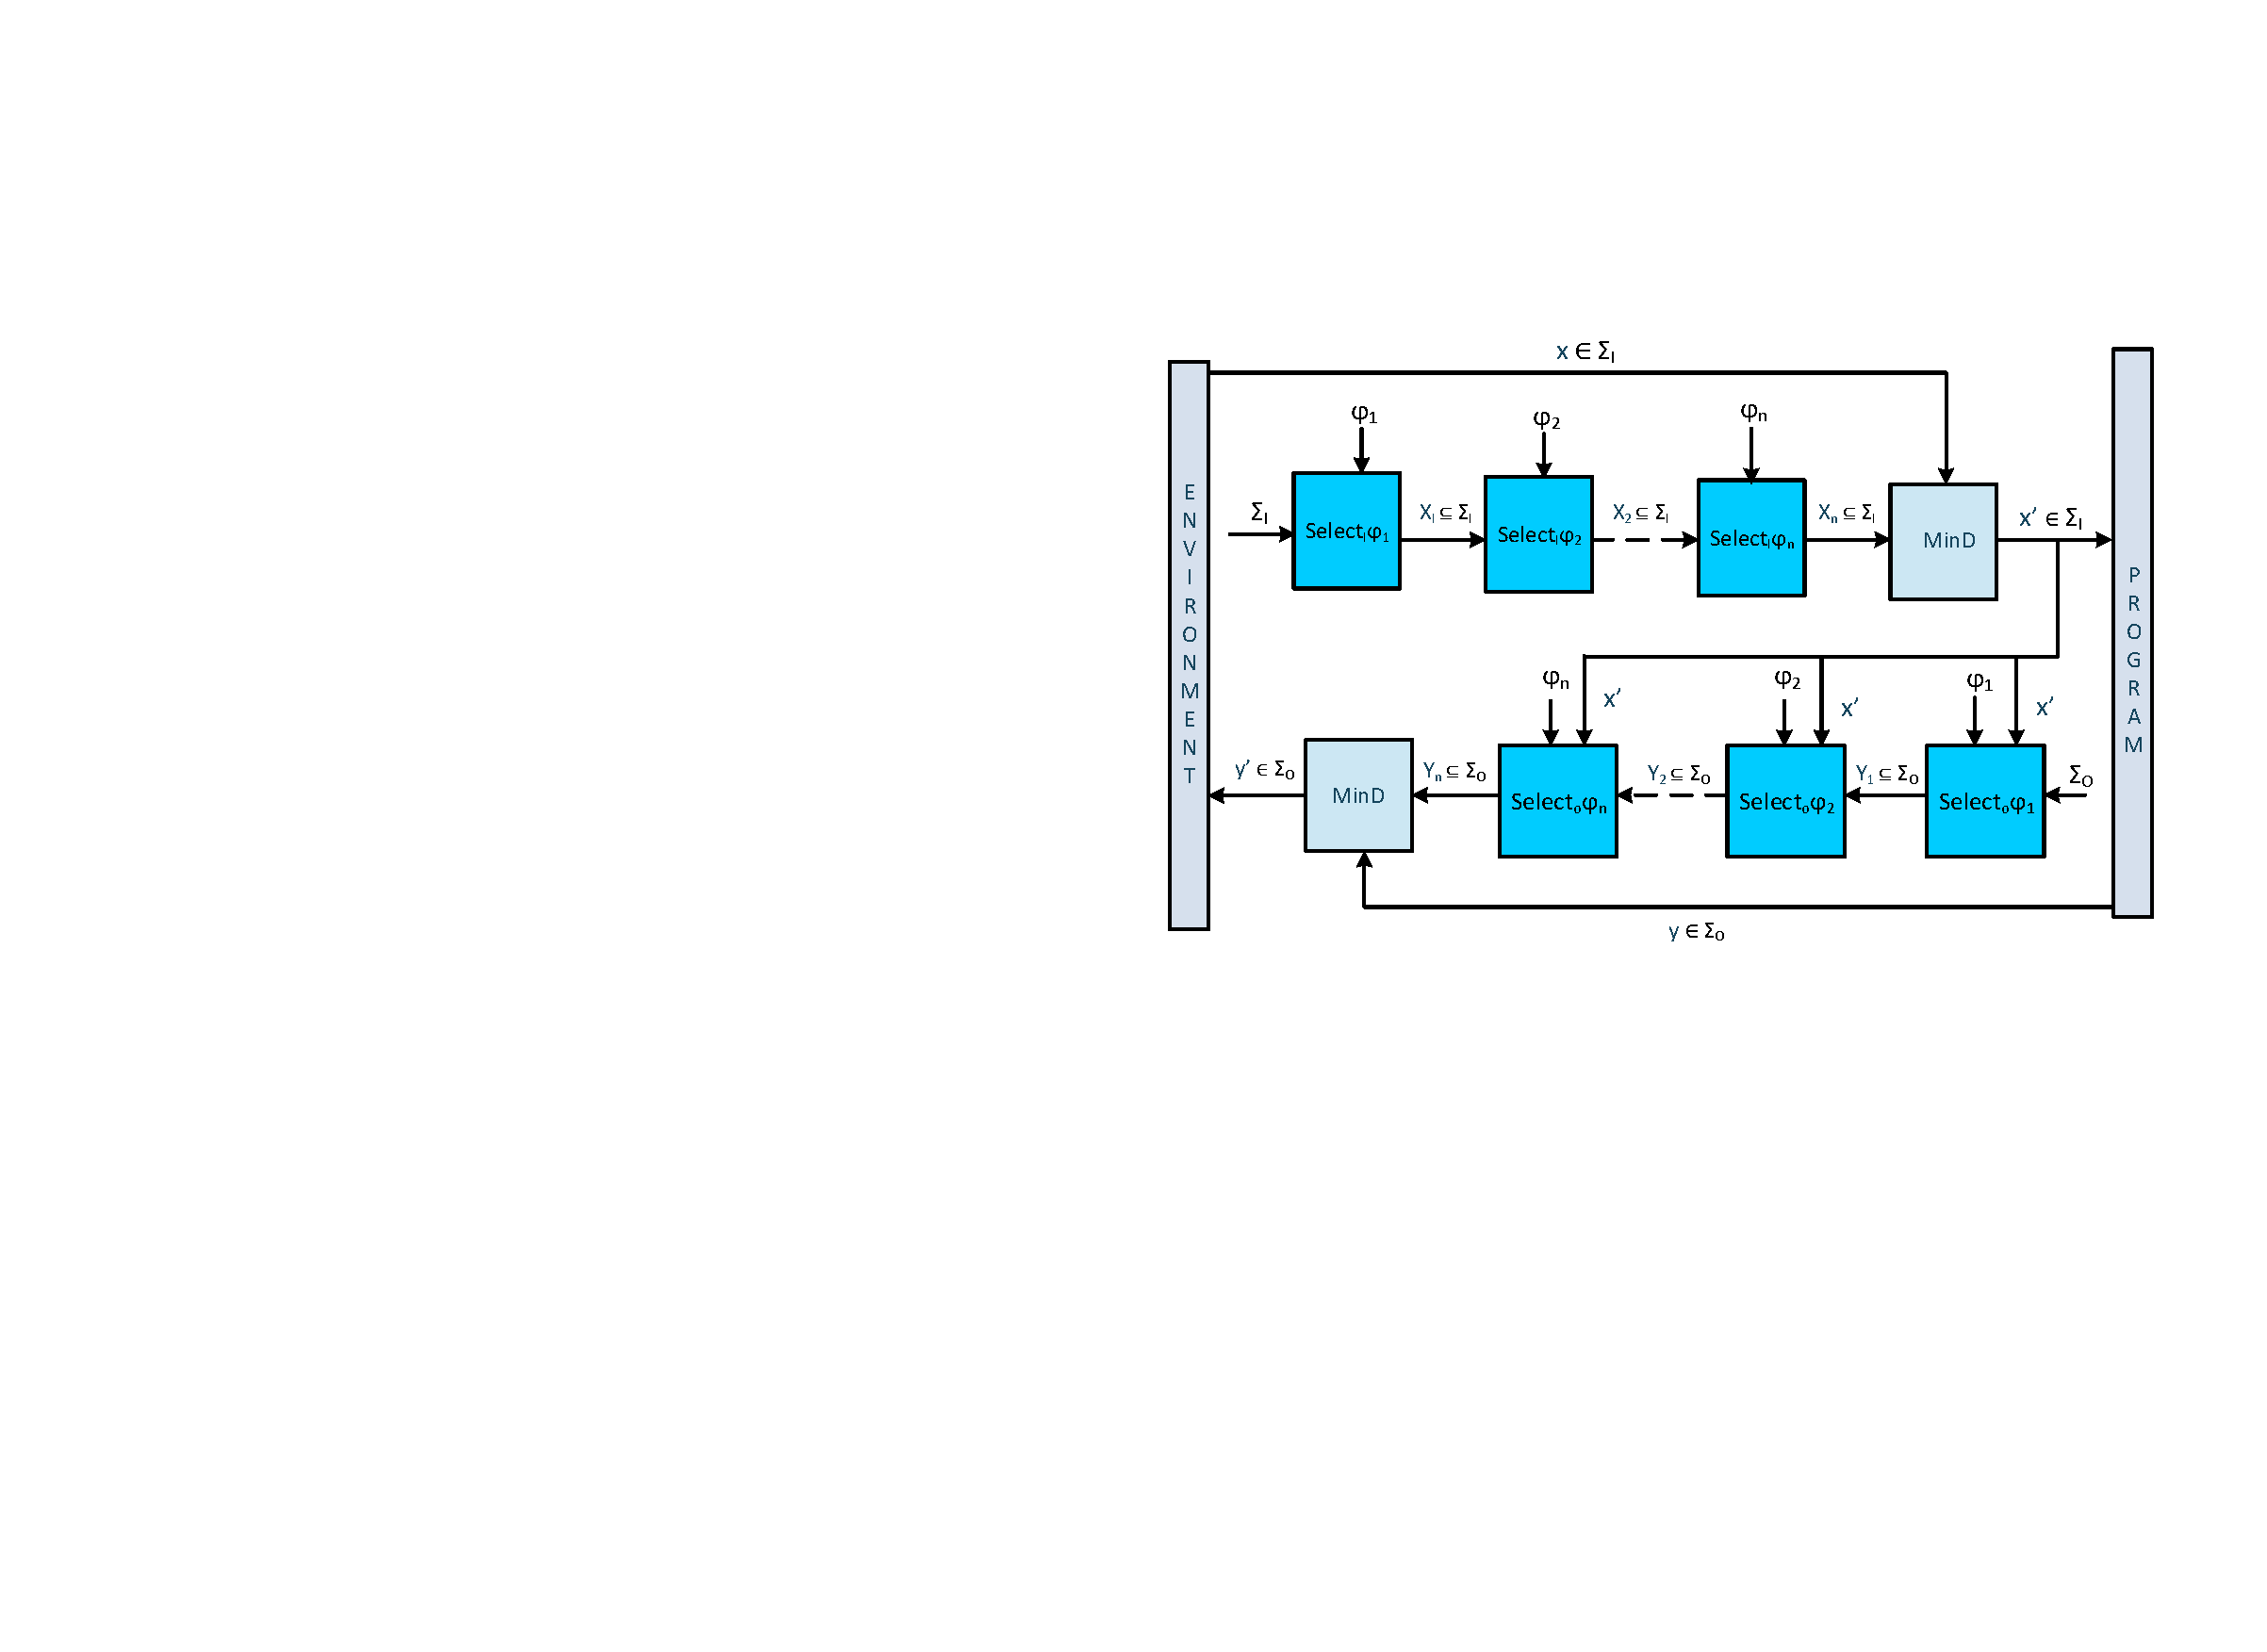
\includegraphics[width=1.1\columnwidth]{fig/serial-composition2-ColourDiagram-cropped5.pdf}
	\captionof{figure}{Incremental Enforcement via Serial Composition using Select functions}
	\label{fig:serialComp2}
\end{SingleColFigure}
%%%%%%%%%%%%%%%%%%%%%%%%%%%%%%%%%%%%%%%%%%%%%%%%%%%%%%%%%%%%%%%%

In serial composition using Select, the input enforcer $\efi$ is implemented by the serial composition of $\selectI()$ followed by MinD(). The input set $\Sigma_I$ is fed to $\selectI()$ in serial to pre-compute a valid input set satisfying all policies. As shown in Figure \ref{def:serialComp2}, $\selectI_{\varphi_{1}}$ produces input set $X_1$ according to policy $\varphi_{1I}$ from input $\Sigma_I$. Similarly, $\selectI_{\varphi_{2}}$ outputs set $X_2$ w.r.t policy $\varphi_{2I}$ from input $X_1$ and so on. The final input set  obtained $X_n$ satisfying all policies $\varphi_1$, $\varphi_2$ $\cdots$ $\varphi_n$ is input to MinD(). Whenever an input $x$ is received from the environment, it is fed to MinD() that selects a minimal edit $x' \in X_n$  such that $\sigma_I \cdot x' $ ($\sigma_I$ already output) satisfies input policies. 

Similarly, the serial composition of output enforcer $\efo$ is implemented with the serial composition of $\selectO()$ followed by MinD(). The output of input enforcer $a'$ along with all possible output $\Sigma_O$ are fed to $\selectO()$ in serial to pre-compute a valid output set satisfying all policies. As shown in Figure \ref{def:serialComp2}, $\selectO_{\varphi_{1}}$ chooses output set $Y_1$ according to policy $\varphi_{1}$ for input $x'$. Similarly, $\selectO_{\varphi_{2}}$ chooses set $Y_2$ according to policy $\varphi_{2}$ from input $Y_1$ and so on. The final output set  obtained $Y_n$ satisfying all policies $\varphi_1$, $\varphi_2$ $\cdots$ $\varphi_n$ is input to MinD(). Whenever an output $y$ is received from the program, it is fed to MinD() that selects a minimal edit $y' \in Y_n$  such that $\sigma \cdot (x',y') $ ($\sigma_I$ already output) satisfies policies. 





%%%%%%%%%%%%%%%%%%%%%%%%%%%%%%%%%%%%%%%%%%%%%%%%%%%%%%%%%%%%%%%%
\begin{definition}[Incremental enforcement via serial composition using select]
	\label{def:serialComp2}
	Given two properties $\varphi_1$ and $\varphi_2$ (where $\varphi_{1I}$ and $\varphi_{2I}$ are their corresponding input policies), we define the enforcement function $\e{\varphi_1} \serial \e{\varphi_2} : \Sigma^* \rightarrow \Sigma^*$ as \efo(\efi($\sigma_I$), $\sigma_O$) where :
	
	
	
	\begin{itemize}
		\item $\efi: \Sigma_I^* \rightarrow \Sigma_I^* $ is defined as:
		
		
		\[
		\begin{array}{rll}
			\hspace{-4em}	\efi(\epsilon_{\Sigma_I})& = \epsilon_{\Sigma_I} \\
			
			\hspace{-4em} \efi(\sigma \cdot a) & = \sigma'_I \cdot MinD(a,\selectI_{\varphi_{2}}(\sigma'_I,(\selectI_{\varphi_{1}}(\sigma'_I,\Sigma_I))))
			
			
		\end{array}
		\]
		~~~~where $\sigma'_I= \efi(\sigma) $.
		
		\vspace{1em}	
		\item $\efo: \Sigma^*_I \times \Sigma^*_O \rightarrow (\Sigma_I \times \Sigma_O)^*$ is defined as:
		\[
		\begin{array}{rll}
			\efo(\epsilon_{\Sigma_I}, \epsilon_{\Sigma_O})& = \epsilon_\Sigma\\
			\hspace{-2em}
			\efo(\sigma_I \cdot x, \sigma_O \cdot y) & = \sigma' \cdot (x,y')
			
		\end{array}
		\]
		~~~~where $\sigma'$ = \efo($\sigma_I$,$\sigma_O$) \\
		$y'= MinD(y,\selectO_{\varphi_2}(\sigma',x,\selectO_{\varphi_1}(\sigma',x,\Sigma_O)))$.	
	\end{itemize}
	
\end{definition}

%%%%%%%%%%%%%%%%%%%%%%%%%%%%%%%%%%%%%%%%%%%%%%%%%%%%%%%%
%%%%%%%%%%%%%%%%%%%%%%%%%%%%%%%%%%%%%%%%%%%%%

Note that the serial composition of enforcers using Select functions always works. That is, given two policies $\varphi_1$, $\varphi_2$ and also $\varphi_1 \cap \varphi_2$ are all enforceable, serial composition of enforcers of $\varphi_1$ and $\varphi_2$ as per the above definition works and the final output obtained will always satisfy $\varphi_1 \cap \varphi_2$. Let us consider input enforcement to understand this (similar reasoning also applies to output enforcement).
As per the serial composition Definition \ref{def:serialComp2}, all possible inputs $\Sigma_I$ are fed to the input enforcers in serial composition\blue{,} and the set obtained (using $\selectI$() ) is a valid one satisfying all input policies ($\varphi_1$and $\varphi_2$ in this case). When a new input word is received, it is input to the MinD() that chooses (if required) a suitable element from the valid set available with it. 

Let us consider the following example to understand this further.

\begin{example}[Serial composition scheme using Select()]
	Let us again consider policies $S_1$ and $S_2$ illustrated in Figure \ref{fig:prop1&2}. 
	Both policies $S_1$ and $S_2$ are enforceable individually. The policy $S_1 \cap S_2$ is also enforceable. 
	Also, when we compose input and output enforcers for these policies in series as per Definition \ref{def:serialComp2}, the final output obtained does satisfy policy $S_1 \cap S_2$. For example consider the word $(100,1) \cdot (110,1) \cdot (011,0)$ to be processed incrementally is shown in Tables \ref{table:EgSerialDef21} and \ref{table:EgSerialDef22}. Whenever any input is given, the MinD() always selects a valid element to input to the output enforcement function, always satisfying all the policies.
\end{example}

\begin{theorem}[Serial composition using select]
	\label{theorem:serial-composition-as-enforcer}
	%	\SP{IMPORTANT: We must be adding about this important result here as a theorem and briefly justify the same:}
	
	{Consider two policies $\varphi_1$, $\varphi_2$ defined as SA, and where $\varphi = \varphi_1 \cap \varphi_2$.}
	%
	{
		If policy $\varphi$ is enforceable, then $\e{\varphi_1} \serial \e{\varphi_2}$ as per Definition \ref{def:serialComp2} is an enforcer for $\varphi$ (satisfies all the constraints as per Definition \ref{def-E-func-constraints}). 
	}
\end{theorem}
The proof of Theorem \ref{theorem:serial-composition-as-enforcer} is given in Appendix \ref{proof:serial-composition-as-enforcer}.The proof is based on induction on the length of the input word $\sigma$.

%%%%%%%%%%%%%%%%%%%%%%%%%%%%%%%%%%%%%
\begin{remark}
	
	Definition \ref{def:serialComp2} supports incrementally adding a new enforcement layer. Whenever another new policy to be enforced $\varphi_i$ is given, we can obtain the input and output select functions for the policy $\varphi_i$ individually, and these can easily be plugged-in to enforce $\varphi_i$ in addition to the previously enforced policies. 
	
\end{remark}
%%%%%%%%%%%%%%%%%%%%%%%%%%%%%%%%%%%%%
%%%%%%%%%%%%%%%%%%%%%%%%%%%%%%%%%%
%%%%%%%%%%%%%%%%%%%%%%%%%%%%%%%%%%%
%

\begin{remark}[ORDER OF COMPOSITION OF ENFORCERS DOES NOT MATTER]
	The order in which the input (resp. output) enforcers are composed, does not affect the final outcome in the proposed incremental enforcement approach. From the definition \ref{def:serialComp2}, we can see that each enforcer from the input set computes the set of all valid events w.r.t its policy, which is fed to the next enforcer in the sequence. The output set produced by the last enforcer in the sequence satisfies all the policies from which one element is chosen by MinD. Thus the order of input (resp. output) enforcers do not matter
	in the proposed incremental enforcement scheme.
\end{remark}

%%%%%%%%%%%%%%%%%%%%%%%%%%%%%%%%
\ignore{
	
	\begin{table*}
		\vspace{-1em}
		\centering
		\resizebox{.9\textwidth}{!}{% <------ Don't forget this %
			\begin{tabular}{|c|c|c|c|c|c|}
				\hline
				$\sigma_I$ & $\sigma_O$ & $X_1 = \selectI_{S1}(\sigma'_I,\Sigma_I)$ & $X' = \selectI_{S2}(\sigma'_I,X_1)$ & $x'= MinD(x,X')$ & $\sigma'_I$  \\
				\hline
				$100$ & $1$ & $\selectI_{S1}(\epsilon_I,\Sigma_I)=\{100,101,010,001,011\}$ & $\selectI_{S2}(\epsilon_I,X_1)=\{100,101,010,001\}$ & $MinD(100,\{100,101,010,001\})=100$ &  $100 $  \\
				\hline
				$100 \cdot 110$ & $1 \cdot 1 $ & $\selectI_{S1}(100,\Sigma_I)=\{100,101,010,001,011\}$ & $\selectI_{S2}(100,X_1)=\{100,101,010,001\}$ & $MinD(110,\{100,101,010,001\})=100$ & $100 \cdot 100 $  \\
				
				\hline
				$100 \cdot 110 \cdot 011$ & $1 \cdot 1 \cdot 0 $ & $\selectI_{S1}(100.100,\Sigma_I)=\{100,101,010,001,011\}$  & $\selectI_{S2}(100\cdot100,X_1)=\{100,101,010,001\}$ & $ MinD(011,\{100,101,010,001\})=001$ &  $100 \cdot 100 \cdot 001$ \\
				
				\hline
			\end{tabular}
		}
		\caption{Serial composition scheme using Select()-input enforcement}
		\label{table:EgSerialDef21}
		
	\end{table*}
	%%%%%%%%%%%%%%%%%%%%%%%%%%%%%%%%
	\begin{table*}
		\vspace{-1em}
		\centering
		\resizebox{.9\textwidth}{!}{% <------ Don't forget this %
			\begin{tabular}{|c|c|c|c|}
				\hline
				$Y' = \selectO_{S1}(\sigma',x',\Sigma_O)$ & $Y''=\selectO_{S2}(\sigma',x',Y')$ & $MinD(y,Y'')$ & $\sigma'$\\
				\hline
				$\selectO_{S1}(\epsilon,100,\Sigma_O)=\{0,1\}$ & $\selectO_{S2}(\epsilon,100,Y')=\{0,1\}$ & $MinD(1,\{0,1\})=1$ & $(100,1)$ \\
				\hline
				$\selectO_{S1}((100,1),100,\Sigma_O)=\{0,1\}$ & $\selectO_{S2}((100,1),100,Y')=\{0,1\}$ & $MinD(1,\{0,1\})=1$ & $(100,1) \cdot (100,1)$ \\
				
				\hline
				$\selectO_{S1}((100,1)\cdot (100,1),001,\Sigma_O)=\{0,1\}$ & $\selectO_{S2}((100,1)\cdot (100,1),001,Y')=\{0,1\}$ & $MinD(0,\{0,1\})=0$ & $(100,1) \cdot (100,1) \cdot (001,0)$\\
				
				\hline
			\end{tabular}
		}
		\caption{Serial composition scheme using Select()-output enforcement}
		\label{table:EgSerialDef22}
		
	\end{table*}
}



